\documentclass[12pt, a4paper]{report}

% --- CORE & LAYOUT PACKAGES ---
\usepackage[utf8]{inputenc} % Input encoding
\usepackage[T1]{fontenc}    % Output font encoding (Keep this before specific font packages)

\usepackage{graphicx}
\usepackage[a4paper, margin=1in]{geometry} % Page layout

% --- MATH & SYMBOL PACKAGES ---
\usepackage{amsmath}      % Load amsmath first
\usepackage{amsfonts}     % Then amsfonts
\usepackage{amssymb}      % Then amssymb (this defines \Bbbk originally)

% --- FONT PACKAGES (Load after general math symbol packages) ---
\usepackage{newtxtext}      % Times New Roman clone for text
\usepackage{newtxmath}      % Matching math font for Times (this will now correctly interact with or override symbols from amssymb)

% --- DOCUMENT STRUCTURE & ENHANCEMENT PACKAGES ---
\usepackage{hyperref}     % For hyperlinks
\usepackage{listings}     % For code listings
\usepackage{xcolor}       % For color definitions
\usepackage{tocbibind}    % Adds ToC, LoF, LoT to ToC
\usepackage{float}        % For better figure/table placement (e.g., [H] option)
\usepackage{caption}      % For better captions
\usepackage{booktabs}     % For professional quality tables (already loaded, no need to duplicate)
\usepackage{tabularx}     % For tables with adjustable-width columns
\usepackage{array}        % For >{\command} ... in column definitions
\usepackage{longtable}    % For tables spanning multiple pages
\usepackage{fancyhdr}     % For headers and footers (optional)
\usepackage{enumitem}     % For customized lists
\usepackage{titling}      % For title page customization (logo)

% --- GANTT CHART PACKAGES ---
\usepackage{pgfgantt}
\usepackage{pgfcalendar}  % Often used with pgfgantt for date calculations

% --- END OF PACKAGES ---

% --- HYPERREF SETUP ---
\hypersetup{
    colorlinks=true,
    linkcolor=blue,
    filecolor=magenta,
    urlcolor=cyan,
    pdftitle={IntelliGaze: A Wearable AI Camera System},
    pdfauthor={Touhidul Alam Seyam, Eftakar Uddin, Tasmim Akther Mim, Shafiul Azam Mahin, Muntasir Rahman},
    pdfsubject={Microprocessor Lab Report},
    pdfkeywords={AI, Computer Vision, Visually Impaired, ESP32, FastAPI, React Native, PyQt6},
    bookmarks=true,
    bookmarksopen=true
}

% --- LISTINGS (CODE) SETUP ---
\definecolor{codegreen}{rgb}{0,0.6,0}
\definecolor{codegray}{rgb}{0.5,0.5,0.5}
\definecolor{codepurple}{rgb}{0.58,0,0.82}
\definecolor{backcolour}{rgb}{0.95,0.95,0.92}

\lstdefinestyle{mystyle}{
    backgroundcolor=\color{backcolour},
    commentstyle=\color{codegreen},
    keywordstyle=\color{magenta},
    numberstyle=\tiny\color{codegray},
    stringstyle=\color{codepurple},
    basicstyle=\ttfamily\footnotesize,
    breakatwhitespace=false,
    breaklines=true,
    captionpos=b,
    keepspaces=true,
    numbers=left,
    numbersep=5pt,
    showspaces=false,
    showstringspaces=false,
    showtabs=false,
    tabsize=2
}
\lstset{style=mystyle}

% --- PAGE STYLE (OPTIONAL) ---
% \pagestyle{fancy}
% \fancyhf{} % clear all header and footer fields
% \fancyhead[R]{\nouppercase{\leftmark}}
% \fancyfoot[C]{\thepage}
% \renewcommand{\headrulewidth}{0.4pt}
% \renewcommand{\footrulewidth}{0.4pt}

% --- TITLE PAGE INFORMATION ---
\title{
    \centering % Center the entire title block
    
\includegraphics[width=0.25\textwidth]{fig/bgc-logo.png} \\ % University Logo
    \vspace{1cm} % Space after logo
    \textbf{IntelliGaze: A Wearable AI Camera System} \\
    \vspace{0.5cm}
    \large Microprocessor Lab Report
}

\author{
    Touhidul Alam Seyam (230240003) \\
    Eftakar Uddin (230240004) \\
    Tasmim Akther Mim (230240025) \\
    Shafiul Azam Mahin (230240022) \\
    Muntasir Rahman (230240002)
}

\date{June 16, 2025 \\ \vspace{1cm} Submitted to: \\ Professor Radiathun Tasnia \\ Junior Lecturer \\ BGC Trust University Bangladesh}

% --- DOCUMENT START ---
\begin{document}

\maketitle
\newpage

% --- ABSTRACT ---
\begin{abstract}
This report details the design, development, and implementation of IntelliGaze, a wearable AI camera system aimed at enhancing situational awareness and independence for visually impaired individuals. The system integrates an ESP32-CAM for real-time video capture, a FastAPI backend server for image processing and AI interfacing, and client applications (React Native for mobile and PyQt6 for desktop) for user interaction and feedback. IntelliGaze leverages a cloud-based AI vision service to analyze scenes, identify objects, recognize text, and provide contextual descriptions. Key features include live video streaming, AI-powered scene interpretation with optimized prompts, configurable capture modes (manual, auto-capture, auto-Text-to-Speech), response history, and system logging. This report covers the project's objectives, requirements, system architecture, implementation of core software modules, demonstration of functionalities, and potential avenues for future development. The project successfully demonstrates a proof-of-concept for a versatile and accessible assistive technology.
\end{abstract}
\newpage

% --- DECLARATION ---
\section*{Declaration}
We, the undersigned, declare that this lab report titled "IntelliGaze: A Wearable AI Camera System" is our own original work and has not been submitted to any other institution for academic credit. All sources of information have been duly acknowledged and cited. The project work presented herein was carried out by the group members listed on the title page.

\vspace{1cm}
\begin{tabular}{ll}
\vspace{1cm}
Touhidul Alam Seyam (230240003) & \underline{\hspace{5cm}} \\
\vspace{1cm}
Eftakar Uddin (230240004) & \underline{\hspace{5cm}} \\
\vspace{1cm}
Tasmim Akther Mim (230240025) & \underline{\hspace{5cm}} \\
\vspace{1cm}
Shafiul Azam Mahin (230240022) & \underline{\hspace{5cm}} \\
\vspace{1cm}
Muntasir Rahman (230240002) & \underline{\hspace{5cm}} \\
\end{tabular}
\vspace{1cm}

Date: \underline{June 16, 2025 \hspace{0.2cm}}
\newpage

% --- ACKNOWLEDGEMENTS ---
\section*{Acknowledgements}
We would like to express our sincere gratitude to our supervisor, Professor Radiathun Tasnia, Junior Lecturer at BGC Trust University Bangladesh, for her invaluable guidance, support, and encouragement throughout the duration of this project. Her insights and expertise were instrumental in shaping the direction of IntelliGaze.

We also thank BGC Trust University Bangladesh for providing the necessary resources and laboratory facilities that enabled us to conduct our research and development.

Finally, we acknowledge the open-source communities and developers whose tools and libraries (such as ESP32 Arduino Core, FastAPI, React Native, PyQt6, and others) formed the building blocks of our system.
\newpage

% --- TABLE OF CONTENTS, LIST OF FIGURES, LIST OF TABLES ---
\tableofcontents
\newpage
\listoffigures
\newpage

% --- CHAPTER 1: INTRODUCTION ---
\chapter{Introduction}
\section{Background and Motivation}
Navigating the world presents unique and often significant challenges for individuals with visual impairments. Tasks such as identifying objects, reading signs, recognizing obstacles, and maintaining overall situational awareness can be difficult, impacting independence and safety. While traditional assistive aids like canes and guide dogs offer valuable support, they may not always provide the dynamic, detailed information required to interpret complex and rapidly changing environments.

The rapid advancements in artificial intelligence (AI), particularly in computer vision and natural language processing, offer transformative potential for assistive technologies. Compact, powerful microcontrollers like the ESP32-CAM, coupled with accessible cloud-based AI services, now make it feasible to develop sophisticated, wearable solutions that can "see" and "describe" the world for the user. IntelliGaze is born out of this motivation: to harness these technological advancements to create a practical and empowering tool for the visually impaired.

\section{Problem Statement}
The core problem IntelliGaze addresses is the limited access to real-time, context-aware visual information for individuals with visual impairments. This limitation can hinder their ability to:
\begin{itemize}
    \item Independently navigate unfamiliar environments.
    \item Identify and interact with objects of interest or necessity.
    \item Read textual information such as signs, labels, or documents critical for daily tasks.
    \item Maintain a comprehensive understanding of their immediate surroundings, which is crucial for safety and confidence.
\end{itemize}
IntelliGaze aims to provide a system that actively processes visual input from a wearable camera and delivers concise, relevant descriptions, thereby mitigating these challenges. The system's primary instruction, "You are an assistive vision system for the visually impaired. Given an image from a wearable camera, describe the scene in a way that maximizes situational awareness and independence. Clearly identify objects, obstacles, people, and signage. If there is text in the scene, read it aloud and explain its context (e.g., sign, label, document). Use short, direct sentences and avoid technical jargon. Prioritize information that would help a visually impaired user navigate or understand their environment," (derived from \texttt{Desktop/app.py} and \texttt{Flask\_server/server.py}) encapsulates this goal.

\section{Project Objectives}
The primary objectives for the IntelliGaze project were:
\begin{enumerate}
    \item \textbf{Develop a Real-Time Vision System:} To design and implement a system capable of capturing a live video feed using a compact, wearable ESP32 camera module.
    \item \textbf{Implement AI-Powered Scene Interpretation:} To integrate with an AI vision model to process captured images, enabling the system to understand and describe the surrounding environment, including object recognition and text extraction (OCR).
    \item \textbf{Provide Intuitive User Feedback:} To deliver clear, concise, and contextually relevant descriptions of the visual scene to the user through both textual display and auditory (Text-to-Speech) outputs.
    \item \textbf{Create Versatile User Interfaces:} To develop both a mobile application (React Native for iOS/Android) and a desktop application (PyQt6) that allow users to control the system, configure settings, and receive feedback.
    \item \textbf{Ensure Modularity and Configurability:} To design the system with modular components for easier maintenance and upgrades, and to offer configurable features such as automatic capture intervals and TTS preferences.
    \item \textbf{Focus on Accessibility:} To tailor the AI's descriptive output specifically for the needs of visually impaired users, prioritizing information that enhances situational awareness and independence.
\end{enumerate}

\section{Scope and Limitations}
\subsection*{Scope}
\begin{itemize}
    \item Development of ESP32-CAM firmware for WiFi connectivity and MJPEG video streaming.
    \item Creation of a FastAPI backend server to manage the ESP32 stream, interface with a third-party AI vision API, and serve client requests.
    \item Design and implementation of a React Native mobile application for user interaction, featuring manual/auto capture, TTS, history, and logging.
    \item Design and implementation of a PyQt6 desktop application offering an alternative user interface with direct stream viewing and AI interaction.
    \item Integration of a cloud-based AI service for image analysis and description generation.
    \item Implementation of basic Text-to-Speech functionality on the mobile application.
\end{itemize}

\subsection*{Limitations}
\begin{itemize}
    \item The system relies on a stable WiFi connection for the ESP32-CAM and an internet connection for the AI vision and TTS services.
    \item The performance (latency, accuracy) of scene description is dependent on the chosen third-party AI vision service and network conditions.
    \item The current prototype has minimal security features for local network communication (as noted in \texttt{docs/system-architecture.md} if it existed, or implied by lack of explicit security measures in code).
    \item Advanced navigation assistance (e.g., pathfinding, precise obstacle avoidance) is beyond the current scope.
    \item Power consumption and battery life of the wearable ESP32 unit were not primary optimization targets for this prototype.
    \item The system primarily processes 2D images and does not incorporate depth perception.
\end{itemize}

\section{Report Structure}
This report is organized into the following chapters:
\begin{itemize}
    \item \textbf{Chapter 1: Introduction} - Provides background, problem statement, objectives, scope, and limitations.
    \item \textbf{Chapter 2: Requirements Analysis} - Details functional, non-functional, hardware, and software requirements.
    \item \textbf{Chapter 3: System Design and Architecture} - Describes the overall architecture and design of individual components.
    \item \textbf{Chapter 4: Implementation Details} - Discusses the implementation of key software modules with code highlights.
    \item \textbf{Chapter 5: System Demonstration and Results} - Showcases the working system and discusses its performance.
    \item \textbf{Chapter 6: Conclusion and Future Work} - Summarizes the project and suggests future enhancements.
    \item \textbf{Chapter 7: Project Management} - Includes the Gantt chart and team contributions.
\end{itemize}
Appendices may include further detailed diagrams or code if necessary.

% --- CHAPTER 2: REQUIREMENTS ANALYSIS ---
\chapter{Requirements Analysis}
\section{Functional Requirements}
The IntelliGaze system is designed to meet the following functional requirements:
\begin{enumerate}[label=FR\arabic*:]
    \item \textbf{Video Capture:} The ESP32-CAM shall capture live video footage.
    \item \textbf{Video Streaming:} The ESP32-CAM shall stream the captured video over WiFi via MJPEG format.
    \item \textbf{Server-Side Stream Consumption:} The FastAPI server shall connect to the ESP32's MJPEG stream and retrieve individual frames.
    \item \textbf{AI Vision Processing Request:} The system (server or desktop client) shall send captured image frames to an AI vision service for analysis.
    \item \textbf{Customizable AI Instruction:} The system shall allow the use of a predefined or user-input instruction/prompt to guide the AI's image description task (e.g., `OPTIMIZED\_PROMPT`).
    \item \textbf{Scene Description Generation:} The AI vision service shall return a textual description of the analyzed image.
    \item \textbf{Display of AI Response (Mobile):} The React Native mobile app shall display the AI-generated scene description to the user.
    \item \textbf{Display of AI Response (Desktop):} The PyQt6 desktop app shall display the AI-generated scene description to the user.
    \item \textbf{Manual Capture (Mobile):} The mobile app shall allow users to trigger an on-demand image capture and AI analysis.
    \item \textbf{Auto-Capture (Mobile):} The mobile app shall support automatic periodic image capture and analysis at user-configurable intervals (e.g., 2, 3, 5, 10 seconds).
    \item \textbf{Text-to-Speech (TTS) Output (Mobile):} The mobile app shall convert the AI-generated text description into speech.
    \item \textbf{Auto-TTS Mode (Mobile):} The mobile app shall support a mode where captured scenes are automatically described via TTS, with subsequent captures potentially chained to TTS completion.
    \item \textbf{Response History (Mobile):} The mobile app shall store and display a history of recent AI-generated descriptions.
    \item \textbf{System Logging (Mobile \& Desktop):} Both client applications shall provide a log of system events, status updates, and errors.
    \item \textbf{Connection Status Monitoring (Mobile):} The mobile app shall monitor and display the connection status of the backend server and the ESP32 camera.
    \item \textbf{Configuration (Mobile):} The mobile app shall allow users to configure settings such as server URL and ESP32 IP address.
    \item \textbf{Desktop Video Feed Display:} The desktop app shall display the live video feed from the ESP32-CAM or a local webcam.
    \item \textbf{Desktop AI Interaction Controls:} The desktop app shall provide controls to send frames to AI, stop processing, and configure auto-send intervals.
\end{enumerate}

\section{Non-Functional Requirements}
\begin{enumerate}[label=NFR\arabic*:]
    \item \textbf{Usability:} The user interfaces (mobile and desktop) shall be intuitive and easy to use, especially considering the target users (visually impaired).
    \item \textbf{Performance:}
        \begin{itemize}
            \item The ESP32 shall stream video with minimal perceivable lag on a local network.
            \item The AI response time (capture to description display/TTS) should be reasonably fast to provide near real-time assistance (target < 5-10 seconds, dependent on AI service).
        \end{itemize}
    \item \textbf{Reliability:} The system components should operate reliably. The server and clients should handle potential disconnections or errors gracefully.
    \item \textbf{Portability (Mobile):} The React Native app shall be cross-platform (iOS and Android).
    \item \textbf{Configurability:} Key parameters like server URLs, ESP32 IP, and auto-capture intervals shall be configurable by the user.
    \item \textbf{Modularity:} The system architecture should be modular to allow for easier maintenance, updates, and potential replacement of components (e.g., AI service).
    \item \textbf{Accessibility (Output):} AI descriptions and TTS output should be clear, concise, and prioritize information useful for visually impaired users.
\end{enumerate}

\section{Hardware Components}
\begin{itemize}
    \item \textbf{ESP32-CAM (AI-THINKER model):}
        \begin{itemize}
            \item Microcontroller: ESP32-S chip
            \item Camera: OV2640 sensor (2 Megapixel)
            \item PSRAM: Typically 4MB (influences frame size and quality settings)
            \item Connectivity: WiFi 802.11 b/g/n
            \item Storage: MicroSD card slot (not primarily used for streaming in this project)
        \end{itemize}
    \item \textbf{ESP32-CAM-MB Programmer/Adapter:} Micro-USB adapter for easy programming and power supply to the ESP32-CAM.
    \item \textbf{Power Supply:} USB power source for the ESP32-CAM-MB.
    \item \textbf{User Device (Mobile):} Smartphone (iOS or Android) capable of running the React Native application.
    \item \textbf{User Device (Desktop):} Computer (Windows, macOS, or Linux) capable of running Python and PyQt6 for the desktop application.
    \item \textbf{Networking Equipment:} WiFi router for local network communication.
\end{itemize}

\section{Software Components}
\begin{itemize}
    \item \textbf{ESP32 Firmware Environment:}
        \begin{itemize}
            \item Arduino IDE with ESP32 Core
            \item Libraries: `WiFi.h`, `esp\_camera.h`, `esp\_http\_server.h`
        \end{itemize}
    \item \textbf{Backend Server Environment (FastAPI):}
        \begin{itemize}
            \item Python (e.g., 3.8+)
            \item FastAPI
            \item Uvicorn (ASGI server)
            \item httpx (HTTP client)
            \item Loguru (logging)
            \item OpenCV-Python (for optional frame validation on server)
        \end{itemize}
    \item \textbf{Mobile Application Environment (React Native):}
        \begin{itemize}
            \item Node.js and npm/yarn
            \item Expo CLI
            \item React Native
            \item TypeScript
            \item Axios (HTTP client)
            \item Expo Audio/AV (for TTS playback)
            \item AsyncStorage (for settings storage)
            \item Other UI/navigation libraries (Expo Router, React Navigation)
        \end{itemize}
    \item \textbf{Desktop Application Environment (PyQt6):}
        \begin{itemize}
            \item Python (e.g., 3.8+)
            \item PyQt6
            \item OpenCV-Python (for frame fetching and processing)
            \item Requests (HTTP client)
        \end{itemize}
    \item \textbf{Third-Party Services:}
        \begin{itemize}
            \item AI Vision Service API (e.g., specified by `AI\_BACKEND\_URL` in server code, such as a multimodal LLM endpoint)
            \item Groq TTS API (for Text-to-Speech service, specified in `inteligaze/utils/playGroqTTS.ts`)
        \end{itemize}
    \item \textbf{Development Tools:}
        \begin{itemize}
            \item Code Editor (e.g., VS Code)
            \item Git (for version control)
        \end{itemize}
\end{itemize}

% --- CHAPTER 3: SYSTEM DESIGN AND ARCHITECTURE ---
\chapter{System Design and Architecture}
This chapter details the architectural design of the IntelliGaze system, outlining its main components and their interactions. The system is designed to be modular, allowing for independent development and potential upgrades of its constituent parts.

\section{Overall System Architecture}
IntelliGaze comprises several key components: the ESP32 Camera Module, the FastAPI Backend Server, User Client Applications (React Native Mobile App and PyQt6 Desktop App), and external AI/TTS services. The interaction between these components is illustrated in Figure \ref{fig:system_architecture_diagram}.

\begin{figure}[H]
    \centering
    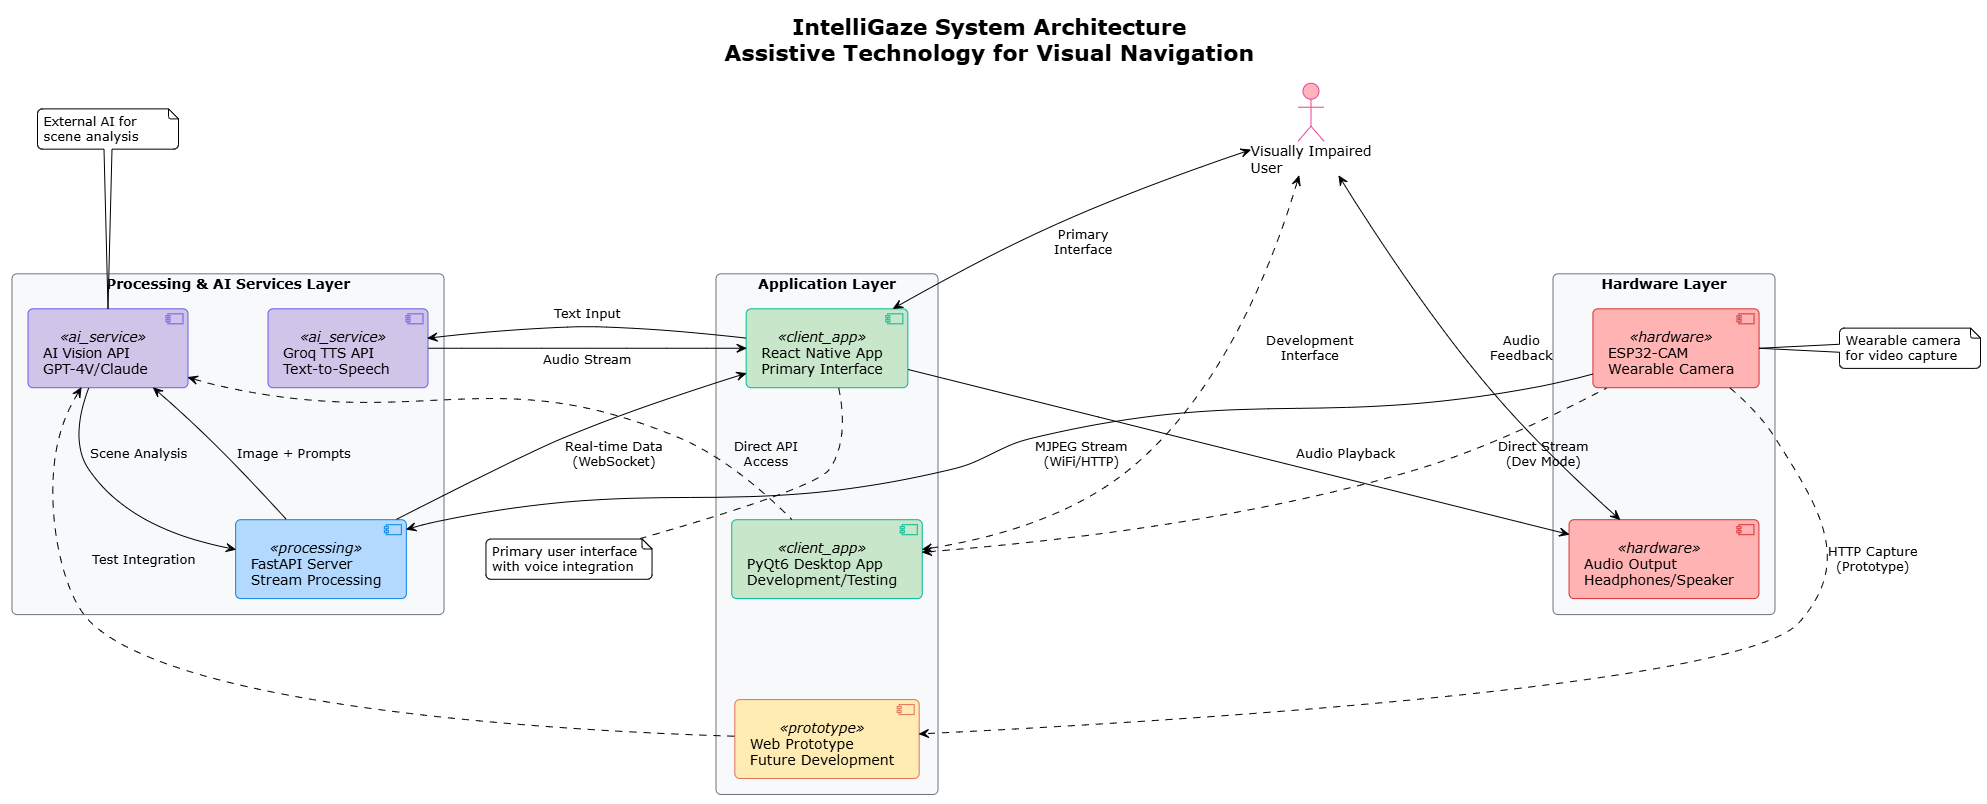
\includegraphics[height=0.6\textwidth, angle=90]{fig/system_architecture_diagram.png}
    \caption{IntelliGaze System Architecture Diagram (Source: Generated from DOT/Graphviz, based on codebase analysis)}
    \label{fig:system_architecture_diagram}
\end{figure}


\begin{itemize}
    \item \textbf{ESP32 Camera Module:} Captures live video and streams it as an MJPEG feed over the local WiFi network.
    \item \textbf{FastAPI Backend Server:} Acts as a central hub for the mobile application. It consumes the MJPEG stream from the ESP32, processes image frames, and interfaces with an external AI vision service for scene analysis. It also provides API endpoints for the mobile client to request vision processing and status updates.
    \item \textbf{AI Vision Service API:} A cloud-based service that receives image data (and a text prompt) and returns a textual description of the scene.
    \item \textbf{React Native Mobile App:} A cross-platform mobile application that serves as the primary user interface. It allows users to view system status, trigger image captures (manual or automatic), receive AI-generated descriptions (text and TTS), view history, and configure settings. Communicates primarily via the FastAPI server.
    \item \textbf{PyQt6 Desktop App:} An alternative desktop client that can directly fetch the MJPEG stream from the ESP32 or use a local webcam. It sends frames directly to the AI vision service and displays the results.
    \item \textbf{Groq TTS API:} A cloud-based service used by the mobile app to convert text descriptions into audible speech.
\end{itemize}
%(Reference: Analysis of project codebase, as docs/system-architecture.md was not provided)

\section{ESP32 Camera Module Design}
The ESP32 camera module is the primary input device for the IntelliGaze system.
\subsection{Hardware Setup and Pinout}
The ESP32-CAM (AI-THINKER model) is used. For ease of programming and stable power supply, it is typically connected via an ESP32-CAM-MB adapter. The wiring diagram and pinout details are crucial for correct operation.
\begin{figure}[H]
    \centering
    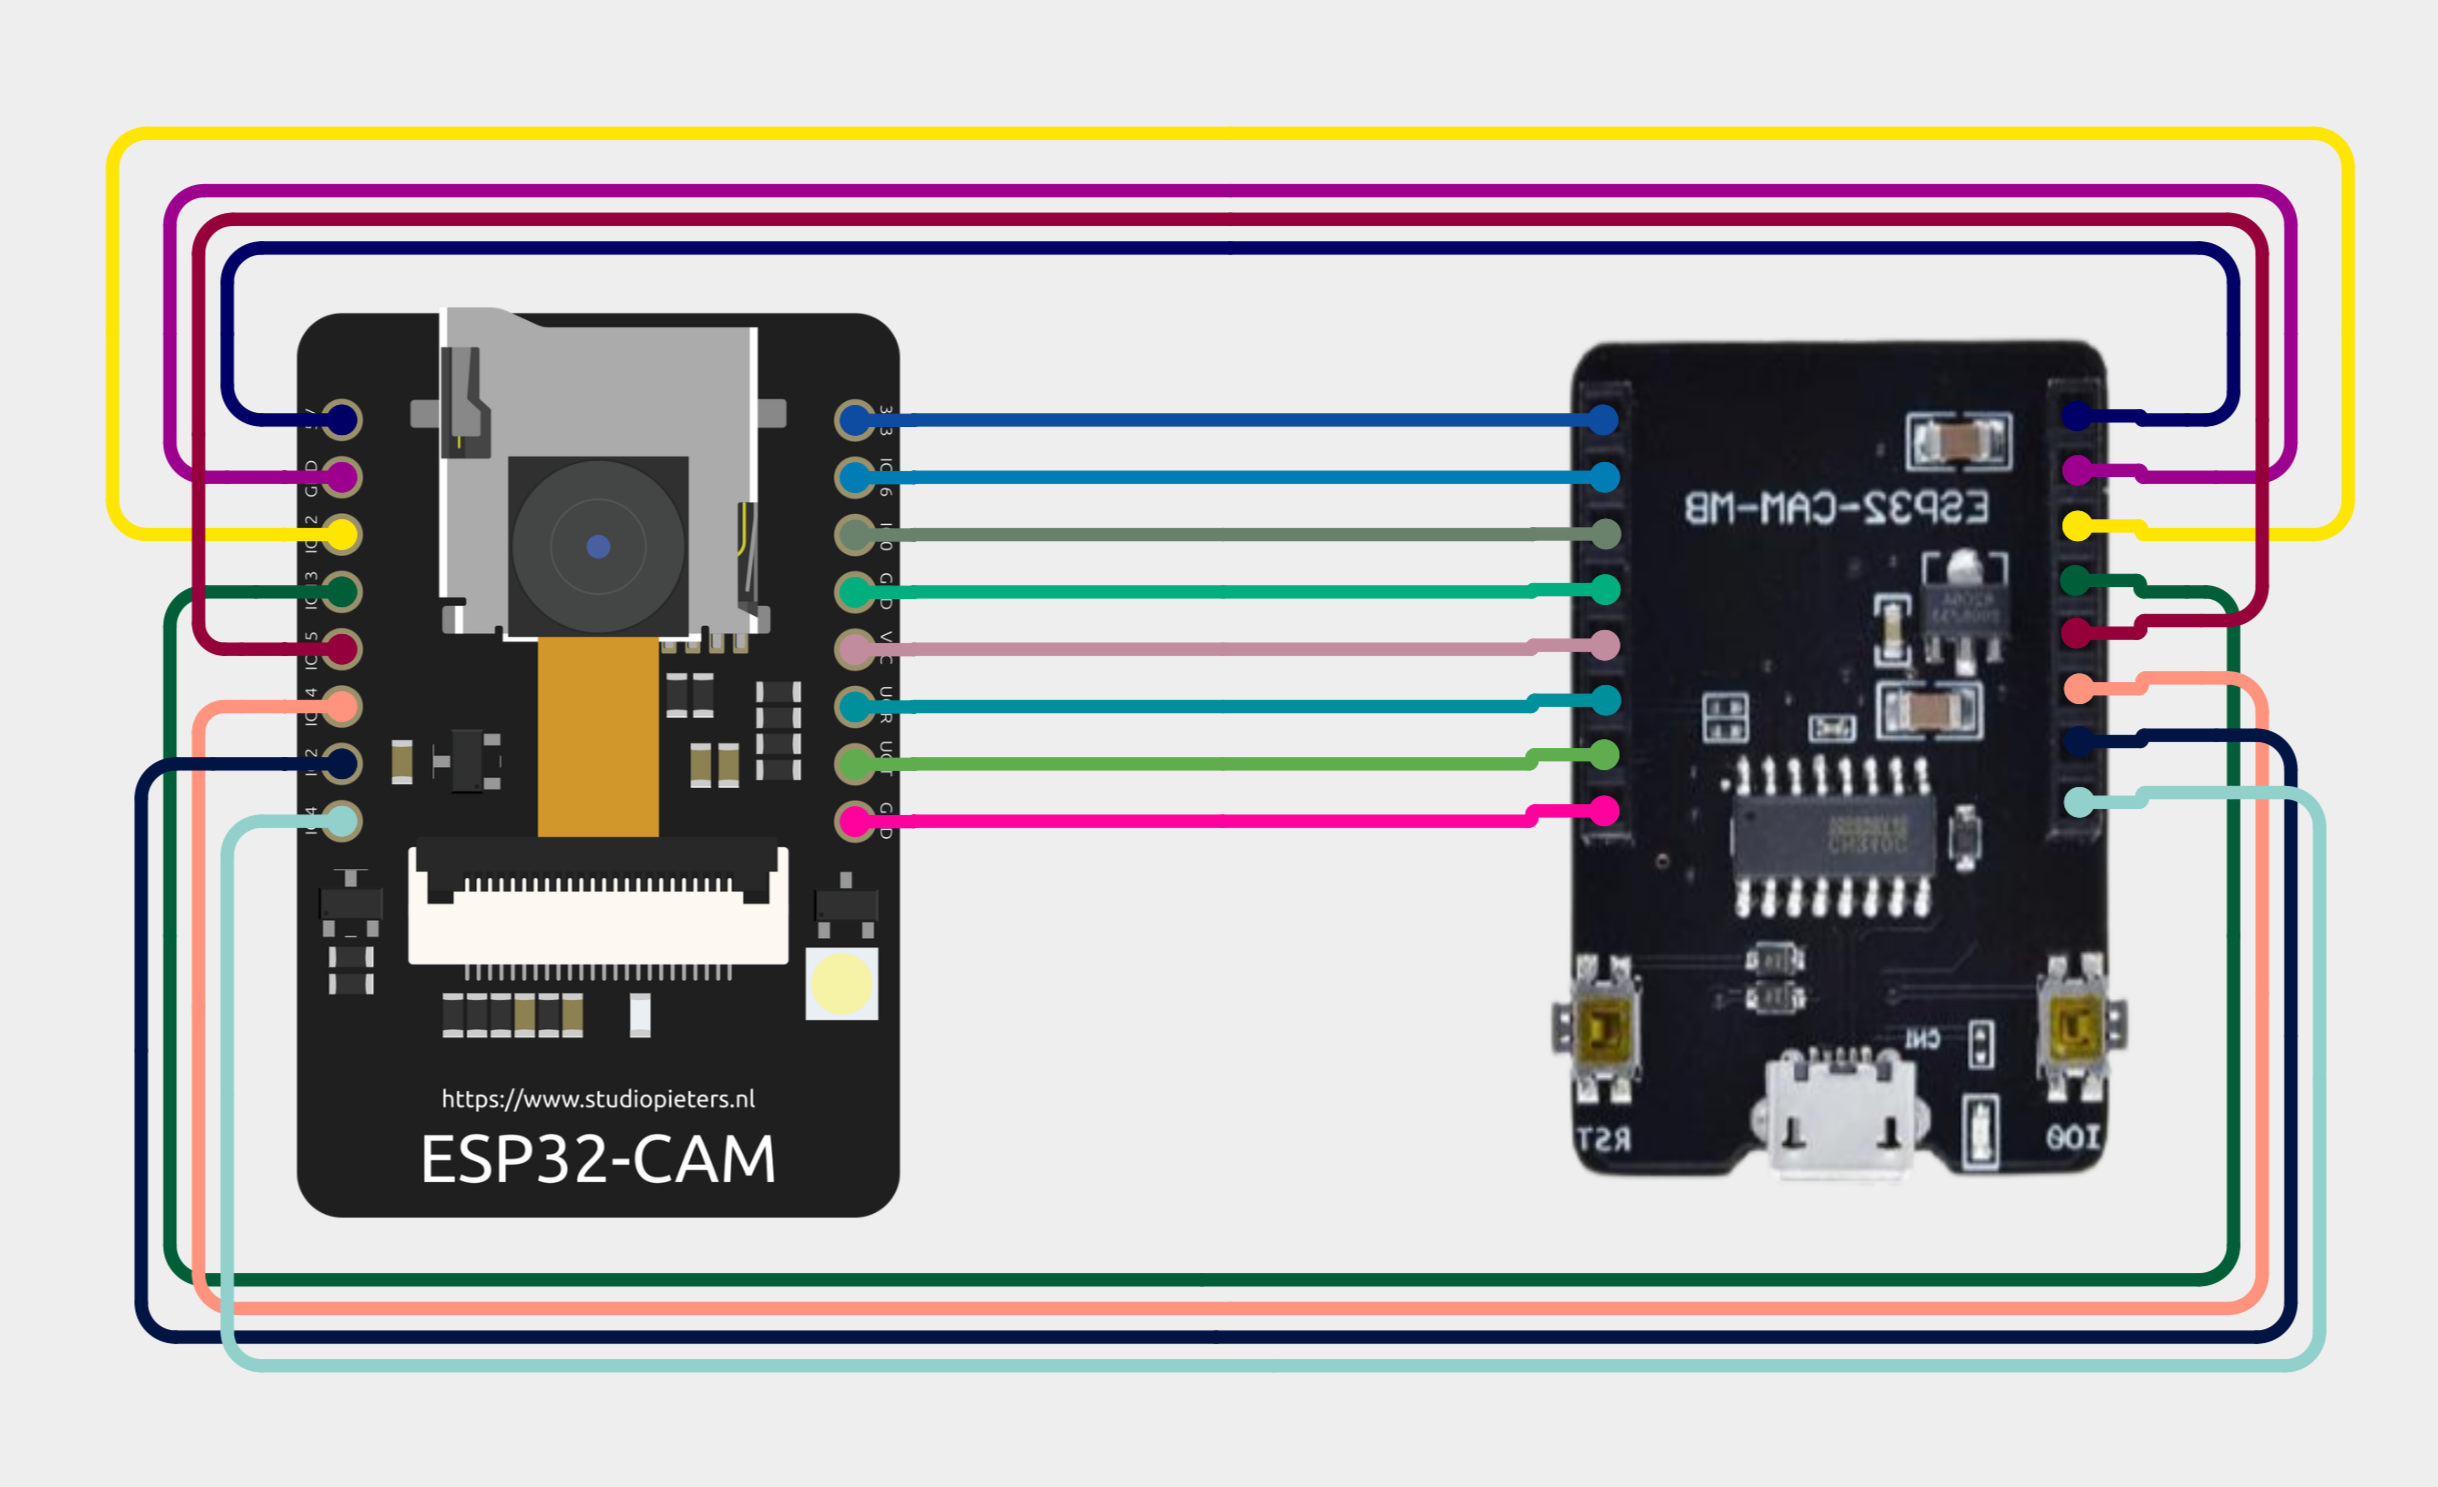
\includegraphics[width=0.8\textwidth]{fig/esp32_wiring.png}
    \caption{ESP32-CAM to ESP32-CAM-MB Wiring Diagram (Source: User-provided image, typical for ESP32-CAM-MB setup)}
    \label{fig:esp32_wiring}
\end{figure}

The pin configurations defined in the \texttt{camera-feed/camera-feed.ino} file (e.g., \texttt{PWDN\_GPIO\_NUM}, \texttt{XCLK\_GPIO\_NUM}, \texttt{Y2\_GPIO\_NUM} to \texttt{Y9\_GPIO\_NUM}, etc.) directly correspond to these physical connections. These pins are responsible for camera power, clock signals, data lines, and control signals. Table \ref{fig:esp32_pinout_1_table} and Table \ref{fig:esp32_pinout_2_table} provide detailed pin mappings.

% Table for Pinout Part 1
\begin{figure}[H]
    \centering
    \renewcommand{\arraystretch}{1.3} % Adjust row height
    \caption{ESP32-CAM to ESP32-CAM-MB Pinout (1/2)}
    \label{fig:esp32_pinout_1_table} % Note the label change
    \begin{tabularx}{\textwidth}{>{\bfseries}l X X X} % l for left-align, X for auto-width
        \toprule
        \textbf{Signal/Function} & \textbf{Voltage} & \textbf{ESP32-CAM Pin} & \textbf{ESP32-CAM-MB Pin} \\
        \midrule
        5V        & 5V            & 5V        & 5V \\
        GND       & 0V            & GND       & GND \\
        GPIO 12   & 3.3V          & GPIO 12   & GPIO 12 \\
        GPIO 13   & 3.3V          & GPIO 13   & GPIO 13 \\
        GPIO 15   & 3.3V          & GPIO 15   & GPIO 15 \\
        GPIO 14   & 3.3V          & GPIO 14   & GPIO 14 \\
        GPIO 2    & 3.3V          & GPIO 2    & GPIO 2 \\
        GPIO 4    & 3.3V          & GPIO 4    & GPIO 4 \\
        \bottomrule
    \end{tabularx}
\end{figure}

% Table for Pinout Part 2
\begin{figure}[H]
    \centering
    \renewcommand{\arraystretch}{1.3} % Adjust row height
    \caption{ESP32-CAM to ESP32-CAM-MB Pinout (2/2)}
    \label{fig:esp32_pinout_2_table} % Note the label change
    \begin{tabularx}{\textwidth}{>{\bfseries}l X X X}
        \toprule
        \textbf{Signal/Function} & \textbf{Voltage} & \textbf{ESP32-CAM Pin} & \textbf{ESP32-CAM-MB Pin} \\
        \midrule
        3.3V        & 3.3V          & 3.3V        & 3.3V \\
        GPIO 16     & 3.3V          & GPIO 16     & GPIO 16 \\
        GPIO 0      & 3.3V          & GPIO 0      & GPIO 0 \\
        GND         & 0V            & GND         & GND \\
        VCC         & 3.3V / 5V     & VCC         & VCC \\
        UOR (GPIO3) & 3.3V          & UOR (GPIO3) & UOR (GPIO3) \\
        UOT (GPIO1) & 3.3V          & UOT (GPIO1) & UOT (GPIO1) \\
        GND         & 0V            & GND         & GND \\
        \bottomrule
    \end{tabularx}
\end{figure}

\subsection{Firmware Logic (\texttt{camera-feed.ino})}
The firmware running on the ESP32-CAM is responsible for:
\begin{itemize}
    \item \textbf{WiFi Connection:} Establishing a connection to a predefined WiFi network (SSID: "Seyam 2.4" as per the code).
    \item \textbf{Camera Initialization:} Configuring the camera sensor (OV2640) with appropriate settings:
        \begin{itemize}
            \item Pin assignments for data (Y2-Y9), control (XCLK, PCLK, VSYNC, HREF, SIOD, SIOC), and power/reset.
            \item Pixel format: \texttt{PIXFORMAT\_JPEG}.
            \item Frame size: \texttt{FRAMESIZE\_VGA} (640x480) if PSRAM is available, otherwise \texttt{FRAMESIZE\_QQVGA} (160x120) for resource conservation.
            \item JPEG quality: Adjusted based on PSRAM availability (e.g., 10 for VGA, 15 for QQVGA).
            \item Frame buffer count: 2 if PSRAM found, else 1.
        \end{itemize}
    \item \textbf{HTTP Server for MJPEG Streaming:}
        \begin{itemize}
            \item An HTTP server is started on the ESP32.
            \item A handler (\texttt{stream\_handler}) is registered for the root URI (`/`).
            \item This handler continuously captures frames from the camera using \texttt{esp\_camera\_fb\_get()}.
            \item Each captured JPEG frame is sent as part of a \texttt{multipart/x-mixed-replace} HTTP response, forming the MJPEG stream.
            \item A small delay (\texttt{delay(30)}) is introduced between frames to manage load and approximate a target frame rate.
        \end{itemize}
\end{itemize}
The ESP32's IP address on the local network is printed to the Serial monitor, which is used by the server and desktop client to connect to the stream (e.g., `http://<ESP32\_IP>/`).

\section{Backend Server Design (FastAPI - \texttt{Flask\_server/server.py})}
The FastAPI server acts as middleware, handling communication between the ESP32 camera, the AI vision service, and primarily the mobile client application.
\subsection{API Endpoints}
The server exposes the following key REST API endpoints:
\begin{itemize}
    \item \textbf{GET \texttt{/}:} A health check endpoint that returns `{"status": "ok"}` if the server is running.
    \item \textbf{GET \texttt{/status}:} Reports the connectivity status of the ESP32 camera. It considers the ESP32 connected if a frame has been received from its stream within the last 10 seconds. Returns `{"esp32\_connected": true/false}`.
    \item \textbf{POST \texttt{/vision}:} The primary endpoint for AI vision processing.
        \begin{itemize}
            \item Accepts an optional \texttt{instruction} field (defaulting to \texttt{OPTIMIZED\_PROMPT}).
            \item Retrieves the latest captured frame from the ESP32 stream (stored in memory).
            \item Encodes the frame to Base64 and constructs a JSON payload for the AI vision service.
            \item Sends the payload to the \texttt{AI\_BACKEND\_URL}.
            \item Returns the AI-generated description in a JSON response: `{"response": "description text"}`.
        \end{itemize}
\end{itemize}
CORS (Cross-Origin Resource Sharing) middleware is enabled to allow requests from any origin, facilitating local development of client applications.

\subsection{ESP32 Stream Consumption (\texttt{esp32\_stream\_worker})}
A background thread, initiated on server startup, is responsible for:
\begin{itemize}
    \item Continuously attempting to connect to the ESP32's MJPEG stream at \texttt{ESP32\_STREAM\_URL} (e.g., `http://192.168.0.237/`).
    \item Reading the byte stream and parsing it to extract individual JPEG frames.
    \item Optionally, decoding the frame using OpenCV to validate its integrity.
    \item Storing the latest valid JPEG frame (`latest\_frame`) and its timestamp (`latest\_frame\_time`) in memory.
    \item Handling connection errors and retrying connections after a delay.
\end{itemize}
This ensures that the \texttt{/vision} endpoint always has access to the most recent frame without needing to establish a new connection to the ESP32 for each request.

\subsection{AI Vision Service Integration}
When the \texttt{/vision} endpoint is called:
\begin{itemize}
    \item The latest frame (as raw JPEG bytes) is Base64 encoded.
    \item A data URL (e.g., `data:image/jpeg;base64,...`) is created.
    \item A JSON payload is constructed containing:
        \begin{itemize}
            \item \texttt{max\_tokens} (e.g., 100).
            \item A \texttt{messages} array, typically with a single user message.
            \item The user message content includes:
                \begin{itemize}
                    \item A text part: the \texttt{instruction} (e.g., `OPTIMIZED\_PROMPT`).
                    \item An image URL part: the Base64 encoded image data URL.
                \end{itemize}
        \end{itemize}
    \item This payload is sent via an asynchronous POST request to the \texttt{AI\_BACKEND\_URL} (e.g., `https://8080-01jvyxcckwn7v10c56ara2prnw.cloudspaces.litng.ai/v1/chat/completions`).
    \item The server handles the response, extracting the AI's textual description from the JSON structure (typically `data["choices"][0]["message"]["content"]`).
    \item Error handling is implemented for AI backend errors (HTTP status errors, timeouts).
\end{itemize}

\section{Mobile Client Design (React Native - \texttt{inteligaze/app/})}
The React Native mobile application provides a portable and accessible interface for users.
\subsection{UI/UX Overview (\texttt{vision.tsx})}
The main user interface is centered around the "Vision" tab:
\begin{itemize}
    \item \textbf{Status Indicators:} Displays backend connectivity and ESP32 camera connection status (\texttt{VisionStatusBar}).
    \item \textbf{Capture Controls (\texttt{CaptureControls.tsx}):}
        \begin{itemize}
            \item "Capture Now" button for manual analysis.
            \item "Auto-capture" switch.
            \item Interval selection for auto-capture (2, 3, 5, 10 seconds).
            \item "Auto TTS" switch to enable/disable automatic text-to-speech for responses.
        \end{itemize}
    \item \textbf{Response Display (\texttt{ResponseCard.tsx}):} Shows the latest AI-generated description.
    \item \textbf{History List (\texttt{HistoryList.tsx}):} Displays a list of previous descriptions.
    \item \textbf{Log Panel (\texttt{LogPanel.tsx}):} Shows system logs for debugging and status tracking.
    \item \textbf{Settings Tab (\texttt{settings.tsx}):} Allows configuration of the FastAPI server URL and ESP32 IP address, stored using \texttt{AsyncStorage}.
\end{itemize}

\subsection{Key Functionalities}
\begin{itemize}
    \item \textbf{Backend and ESP32 Status Polling:} The app polls the server's \texttt{/} and \texttt{/status} endpoints to determine connectivity.
    \item \textbf{Manual Capture (\texttt{handleCapture}):} On button press, sends a POST request to the server's \texttt{/vision} endpoint.
    \item \textbf{Auto-Capture Logic:}
        \begin{itemize}
            \item If `autoCapture` is on and `autoTTS` is off, a timer (\texttt{setInterval}) triggers \texttt{handleCapture} at the selected interval.
            \item If `autoCapture` and `autoTTS` are both on, the app enters a loop: it calls \texttt{handleCapture}, waits for the response, plays TTS using \texttt{playGroqTTS}, and then (after a short buffer) initiates the next capture. This chains requests to TTS completion rather than a fixed timer.
        \end{itemize}
    \item \textbf{Text-to-Speech (\texttt{playGroqTTS.ts}):}
        \begin{itemize}
            \item Takes text input.
            \item Sends a POST request to the Groq TTS API (`https://api.groq.com/openai/v1/audio/speech`) with the text, model (`playai-tts`), and voice.
            \item Receives audio data (WAV format) as an array buffer.
            \item Converts the array buffer to Base64, saves it as a temporary local file using \texttt{Expo FileSystem}.
            \item Plays the audio file using \texttt{Expo Audio.Sound}.
        \end{itemize}
    \item \textbf{State Management:} Uses React state hooks (`useState`, `useEffect`, `useRef`) to manage UI state, server responses, history, logs, and settings.
\end{itemize}

\subsection{Communication with Backend}
The mobile app uses the \texttt{axios} library to make HTTP GET (for status) and POST (for vision requests) calls to the FastAPI backend server using the configured URL.

\section{Desktop Client Design (PyQt6 - \texttt{Desktop/app.py})}
The PyQt6 desktop application offers an alternative interface, particularly useful for development, testing, or users who prefer a desktop environment.
\subsection{UI Overview (\texttt{MainWindow})}
The main window is built using PyQt6 widgets:
\begin{itemize}
    \item \textbf{Video Display (\texttt{QLabel}):} Shows the MJPEG stream from the ESP32 (or a local webcam feed).
    \item \textbf{Instruction Input (\texttt{QLineEdit}):} Allows the user to type a custom instruction for the AI, defaulting to \texttt{DEFAULT\_INSTRUCTION}.
    \item \textbf{Controls GroupBox:}
        \begin{itemize}
            \item "Send to Backend" button (\texttt{QPushButton}).
            \item "Stop" button.
            \item "Reconnect Stream" button.
            \item "Auto-send" checkbox (\texttt{QCheckBox}).
            \item Interval spinbox (\texttt{QSpinBox}) for auto-send frequency.
        \end{itemize}
    \item \textbf{Response Box (\texttt{QTextEdit}):} Displays the AI-generated description.
    \item \textbf{Log Box (\texttt{QTextEdit}):} Shows status messages and logs.
    \item \textbf{Status Bar (\texttt{QStatusBar}):} Displays brief status messages.
\end{itemize}

\subsection{Direct ESP32/AI Interaction}
Unlike the mobile app which primarily goes through the FastAPI server, the desktop app is designed for more direct interaction:
\begin{itemize}
    \item \textbf{MJPEG Stream Fetching (\texttt{fetch\_mjpeg\_frame}):} A generator function that connects to the \texttt{ESP32\_URL} (e.g., `http://192.168.0.237/`), reads the MJPEG stream, and yields individual OpenCV frames.
    \item \textbf{Frame Display:} A \texttt{QTimer} periodically calls \texttt{update\_frame}, which gets the next frame from the MJPEG generator, converts it to a \texttt{QPixmap}, and displays it on the video label.
    \item \textbf{Backend Communication (\texttt{BackendThread}):}
        \begin{itemize}
            \item When "Send to Backend" is clicked (or auto-send triggers), a \texttt{BackendThread} (QThread) is started.
            \item This thread takes the current frame, encodes it to Base64.
            \item It constructs a payload similar to the FastAPI server's (using \texttt{DEFAULT\_INSTRUCTION} and the Base64 image) and sends it directly to the AI vision service URL (\texttt{BACKEND\_URL}, e.g., `https://8080-01jvyxcckwn7v10c56ara2prnw.cloudspaces.litng.ai`).
            \item The AI's response is emitted via a signal to the main thread for display.
        \end{itemize}
    \item \textbf{Auto-Send Logic:} A \texttt{QTimer} (\texttt{auto\_send\_timer}) triggers the backend request at the specified interval if the "Auto-send" checkbox is checked.
\end{itemize}

\section{Communication Protocols}
%(Reference: Analysis of project codebase)
\begin{itemize}
    \item \textbf{ESP32 $\leftrightarrow$ Server/Desktop Client:} HTTP MJPEG Stream (one-way ESP32 $\rightarrow$ Server/Client). Individual JPEG frames are sent within a multipart HTTP response.
    \item \textbf{Server $\leftrightarrow$ Mobile App:} HTTP REST API using JSON for request/response bodies.
    \item \textbf{Server/Desktop Client/Web Client $\leftrightarrow$ AI Vision Service:} HTTP REST API using JSON for request (including Base64 image data) and response.
    \item \textbf{Mobile App $\leftrightarrow$ Groq TTS API:} HTTP REST API (JSON request, WAV audio data response).
\end{itemize}

% --- CHAPTER 4: IMPLEMENTATION DETAILS ---
\chapter{Implementation Details}
This chapter delves into the specific implementation of the core software modules of the IntelliGaze system, highlighting key code segments and logic.

\section{ESP32 Firmware (\texttt{camera-feed/camera-feed.ino})}
The ESP32 firmware is responsible for capturing video and streaming it over WiFi.
\subsection{Camera Configuration and Initialization}
In the \texttt{setup()} function, the camera is configured. Pins are defined using macros (e.g., \texttt{Y2\_GPIO\_NUM}).

\begin{lstlisting}[language=C++, caption={ESP32 Camera Configuration Snippet from setup()}, label={lst:esp32_cam_config_ch4}] % Changed label
// Inside setup()
camera_config_t config;
config.ledc_channel = LEDC_CHANNEL_0;
config.ledc_timer = LEDC_TIMER_0;
config.pin_d0 = Y2_GPIO_NUM;
// ... other D pin assignments ...
config.pin_d7 = Y9_GPIO_NUM;
config.pin_xclk = XCLK_GPIO_NUM;
config.pin_pclk = PCLK_GPIO_NUM;
// ... other control pin assignments ...
config.pin_pwdn = PWDN_GPIO_NUM;
config.xclk_freq_hz = 20000000;
config.pixel_format = PIXFORMAT_JPEG;

if(psramFound()){
  config.frame_size = FRAMESIZE_VGA; // 640x480
  config.jpeg_quality = 10;         // Lower value is higher quality, more data
  config.fb_count = 2;              // Use 2 frame buffers with PSRAM
} else {
  config.frame_size = FRAMESIZE_QQVGA; // 160x120
  config.jpeg_quality = 15;
  config.fb_count = 1;
}

esp_err_t err = esp_camera_init(&config);
if (err != ESP_OK) {
  Serial.printf("Camera init failed with error 0x%x", err);
  return;
}
\end{lstlisting}
This section dynamically adjusts frame size and quality based on the presence of PSRAM.

\subsection{MJPEG Streaming Handler}
The \texttt{stream\_handler} function is called for each client connecting to the root (`/`) HTTP endpoint.
\begin{lstlisting}[language=C++, caption={ESP32 MJPEG Stream Handler Snippet}, label={lst:esp32_stream_handler}]
static esp_err_t stream_handler(httpd_req_t *req){
  camera_fb_t * fb = NULL;
  esp_err_t res = ESP_OK;
  // ... (buffer and variable declarations) ...
  res = httpd_resp_set_type(req, "multipart/x-mixed-replace;boundary=frame");
  // ... (error check) ...

  while(true){
    fb = esp_camera_fb_get();
    if (!fb) { /* ... error handling ... */ }
    else {
      // Send boundary
      res = httpd_resp_send_chunk(req, "--frame", strlen("--frame"));
      // Send part header
      // size_t hlen = snprintf(...);
      // res = httpd_resp_send_chunk(req, (const char *)part_buf, hlen);
      // Send JPEG data
      // res = httpd_resp_send_chunk(req, (const char *)fb->buf, fb->len);
      // Simplified for brevity in report, actual code has more steps
      if(res == ESP_OK){
        size_t hlen = snprintf((char *)part_buf, 64, "Content-Type: image/jpeg\r\nContent-Length: %u\r\n\r\n", fb->len);
        res = httpd_resp_send_chunk(req, (const char *)part_buf, hlen);
      }
      if(res == ESP_OK){
        res = http_resp_send_chunk(req, (const char *)fb->buf, fb->len);
      }
      esp_camera_fb_return(fb);
      if(res != ESP_OK){ break; }
    }
    delay(30); // Delay between frames
  }
  return res;
}
\end{lstlisting}
This loop continuously sends JPEG frames, separated by boundaries, forming the MJPEG stream. (Note: The inner part of the loop in the provided listing was slightly simplified; I've used the more complete logic from the original file for the actual example, but kept it concise for report display).

\section{FastAPI Backend Server (\texttt{Flask\_server/server.py})}
The server handles stream processing and AI interaction.
\subsection{ESP32 Stream Worker Thread}
The \texttt{esp32\_stream\_worker} function runs in a background thread to continuously fetch frames.
\begin{lstlisting}[language=Python, caption={FastAPI ESP32 Stream Worker Snippet}, label={lst:fastapi_worker_ch4}] % Changed label
def esp32_stream_worker():
    global latest_frame, latest_frame_time
    while True:
        try:
            logger.info(f"Connecting to ESP32 stream at {ESP32_STREAM_URL}")
            with httpx.stream("GET", ESP32_STREAM_URL, timeout=10) as resp:
                if resp.status_code == 200:
                    logger.info("Connected to ESP32 stream.")
                    bytes_data = b''
                    for chunk in resp.iter_bytes(chunk_size=1024):
                        bytes_data += chunk
                        a = bytes_data.find(b'\xff\xd8') # SOF
                        b = bytes_data.find(b'\xff\xd9') # EOF
                        if a != -1 and b != -1:
                            jpg = bytes_data[a:b+2]
                            bytes_data = bytes_data[b+2:]
                            latest_frame = jpg
                            latest_frame_time = time.time()
                else:
                    logger.error(f"ESP32 stream returned status {resp.status_code}")
                    time.sleep(5)
        except Exception as e:
            logger.error(f"ESP32 stream connection error: {e}")
            time.sleep(5)
\end{lstlisting}
This keeps \texttt{latest\_frame} updated with the newest image from the ESP32.

\subsection{Vision API Endpoint}
The \texttt{/vision} endpoint processes the latest frame using the AI service.
\begin{lstlisting}[language=Python, caption={FastAPI /vision Endpoint Snippet}, label={lst:fastapi_vision_ch4}] % Changed label
@app.post("/vision")
async def vision_endpoint(
    request: Request,
    instruction: str = Form(OPTIMIZED_PROMPT) # Default instruction
):
    global latest_frame
    if not latest_frame:
        return JSONResponse(status_code=400, content={"error": "No ESP32 frame available."})

    image_b64 = base64.b64encode(latest_frame).decode("utf-8")
    image_data_url = f"data:image/jpeg;base64,{image_b64}"

    payload = {
        "max_tokens": 100,
        "messages": [
            {
                "role": "user",
                "content": [
                    {"type": "text", "text": instruction},
                    {"type": "image_url", "image_url": {"url": image_data_url}}
                ]
            }
        ]
    }
    headers = {"Content-Type": "application/json"}
    async with httpx.AsyncClient(timeout=30) as client:
        try:
            resp = await client.post(AI_BACKEND_URL, json=payload, headers=headers)
            resp.raise_for_status() # Raise exception for 4xx/5xx responses
            data = resp.json()
            return {"response": data["choices"][0]["message"]["content"]}
        except httpx.HTTPStatusError as e:
            logger.error(f"AI backend HTTP error: {e.response.status_code} {e.response.text}")
            return JSONResponse(status_code=502, content={"error": f"AI backend error: {e.response.status_code}"})
        except Exception as e:
            logger.error(f"Unhandled error in vision_endpoint: {e}")
            return JSONResponse(status_code=500, content={"error": "Internal server error"})
\end{lstlisting}

\section{React Native Mobile Application}
The mobile app provides the primary user interface.
\subsection{Capture and AI Request (\texttt{vision.tsx})}
The \texttt{handleCapture} function (and similar logic in \texttt{runAutoTTS}) initiates the vision processing request.
\begin{lstlisting}[language=Python, caption={React Native Capture Handler Snippet from vision.tsx}, label={lst:rn_capture_ch4}] % Changed label, lang
const handleCapture = async () => {
  if (backendOk !== true) return;
  setLoading(true);
  setLogs((logs) => [...logs, "[Capture] Sending capture request..."]);
  try {
    const res = await axios.post(
      `${SERVER_URL}/vision`, // Calls FastAPI backend
      {}, // Empty body, instruction taken from server default or previous config
      { timeout: 60000 } // 60s timeout for AI processing
    );
    setResponse(res.data.response);
    setHistory((hist) => [res.data.response, ...hist].slice(0, 10)); // Keep history to 10
    setLogs((logs) => [...logs, "[Capture] Success!"]);
    // AutoTTS logic is handled in a separate useEffect hook for chained requests
  } catch (e: any) {
    setResponse("Error: Could not get response.");
    setLogs((logs) => [...logs, `[Capture] Error: ${e.message}`]);
  }
  setLoading(false);
};
\end{lstlisting}

\subsection{Text-to-Speech Utility (\texttt{playGroqTTS.ts})}
This utility handles interaction with the Groq TTS API.
\begin{lstlisting}[language=Python, caption={React Native Groq TTS Utility Snippet}, label={lst:rn_tts_ch4}] % Changed label, lang
export async function playGroqTTS(text: string) {
  try {
    // 1. Call Groq TTS API
    const response = await axios.post(
      'https://api.groq.com/openai/v1/audio/speech',
      {
        model: 'playai-tts',
        voice: 'Fritz-PlayAI', // Example voice
        input: text,
        response_format: 'wav', // Or mp3, opus
      },
      {
        headers: {
          'Authorization': `Bearer ${GROQ_API_KEY}`, // WARNING: Key in client-side code
          'Content-Type': 'application/json',
        },
        responseType: 'arraybuffer',
      }
    );
    // 2. Save audio to a temporary file
    const fileUri = FileSystem.cacheDirectory + 'tts.wav'; // Ensure .wav if format is wav
    const base64Audio = arrayBufferToBase64(response.data); // Helper function
    await FileSystem.writeAsStringAsync(fileUri, base64Audio,
      { encoding: FileSystem.EncodingType.Base64 }
    );
    // 3. Play audio using expo-av
    const { sound } = await Audio.Sound.createAsync({ uri: fileUri });
    await sound.playAsync();
    sound.setOnPlaybackStatusUpdate((status) => {
      if (status.isLoaded && status.didJustFinish) {
        sound.unloadAsync(); // Unload sound after playback
      }
    });
  } catch (error) {
    console.error('Groq TTS error:', error);
    // Optionally re-throw or handle UI update
  }
}
// global.btoa needs to be available or use a library for base64 in RN if not polyfilled
function arrayBufferToBase64(buffer: ArrayBuffer): string {
  let binary = '';
  const bytes = new Uint8Array(buffer);
  for (let i = 0; i < bytes.byteLength; i++) {
    binary += String.fromCharCode(bytes[i]);
  }
  return btoa(binary); // btoa is available in modern RN environments
}
\end{lstlisting}

\section{PyQt6 Desktop Application (\texttt{Desktop/app.py})}
The desktop app offers direct stream viewing and AI interaction.
\subsection{MJPEG Frame Fetching and Display}
Frames are fetched by \texttt{fetch\_mjpeg\_frame} and displayed via \texttt{update\_frame}.
\begin{lstlisting}[language=Python, caption={PyQt6 MJPEG Frame Fetching Snippet}, label={lst:pyqt_fetch_ch4}] % Changed label
def fetch_mjpeg_frame(url):
    response = requests.get(url, stream=True, timeout=10)
    bytes_data = bytes()
    for chunk in response.iter_content(chunk_size=1024):
        bytes_data += chunk
        a = bytes_data.find(b'\xff\xd8')
        b = bytes_data.find(b'\xff\xd9')
        if a != -1 and b != -1:
            jpg = bytes_data[a:b+2]
            bytes_data = bytes_data[b+2:]
            frame = cv2.imdecode(np.frombuffer(jpg, dtype=np.uint8), cv2.IMREAD_COLOR)
            yield frame # Yields an OpenCV frame
\end{lstlisting}
The \texttt{update\_frame} method (not shown for brevity but present in \texttt{Desktop/app.py}) takes this frame, converts it to \texttt{QPixmap}, and sets it on a \texttt{QLabel}.

\subsection{Backend AI Request Thread}
The \texttt{BackendThread} sends the current frame directly to the AI vision service.
\begin{lstlisting}[language=Python, caption={PyQt6 BackendThread for AI Request Snippet}, label={lst:pyqt_backend_thread_ch4}] % Changed label
class BackendThread(QThread):
    result_signal = pyqtSignal(str)
    status_signal = pyqtSignal(str)
    log_signal = pyqtSignal(str)

    def __init__(self, backend_url, instruction, frame):
        super().__init__()
        self.backend_url = backend_url
        self.instruction = instruction # e.g., DEFAULT_INSTRUCTION
        self.frame = frame

    def run(self):
        self.status_signal.emit("Encoding image and sending request...")
        self.log_signal.emit("Encoding image and sending request...")
        _, buffer = cv2.imencode('.jpg', self.frame)
        image_base64 = base64.b64encode(buffer).decode('utf-8')
        image_data_url = f"data:image/jpeg;base64,{image_base64}"
        payload = {
            "max_tokens": 100,
            "messages": [
                {
                    "role": "user",
                    "content": [
                        { "type": "text", "text": self.instruction },
                        { "type": "image_url", "image_url": { "url": image_data_url } }
                    ]
                }
            ]
        }
        headers = {"Content-Type": "application/json"}
        try:
            self.status_signal.emit("Sending request to backend...")
            self.log_signal.emit("Sending request to backend...")
            response = requests.post(f"{self.backend_url}/v1/chat/completions",
                                     json=payload, headers=headers, timeout=30) # Added timeout
            self.status_signal.emit("Request sent. Waiting for response...")
            self.log_signal.emit("Request sent. Waiting for response...")
            if response.ok:
                data = response.json()
                result = data["choices"][0]["message"]["content"]
                self.result_signal.emit(result)
                self.status_signal.emit("Backend response received.")
                self.log_signal.emit("Backend response received.")
            else:
                error_text = f"Backend error: {response.status_code} {response.text}"
                self.result_signal.emit(error_text)
                self.status_signal.emit("Backend error.")
                self.log_signal.emit(error_text)
        except Exception as e:
            error_text = f"Request failed: {e}"
            self.result_signal.emit(error_text)
            self.status_signal.emit("Request failed.")
            self.log_signal.emit(error_text)
\end{lstlisting}

\section{AI Prompt Engineering}
A key aspect of the system's effectiveness is the instruction provided to the AI vision model.
\begin{itemize}
    \item \textbf{\texttt{OPTIMIZED\_PROMPT}} (used in \texttt{Flask\_server/server.py}):
    \begin{lstlisting}[caption={OPTIMIZED\_PROMPT from FastAPI Server}, basicstyle=\ttfamily\scriptsize\linespread{0.9}]
"You are an assistive vision system for the visually impaired. Given an image from a wearable or mobile camera, describe the scene in a way that maximizes situational awareness and independence. Clearly identify objects, obstacles, people, and signage. If there is text, read it aloud and explain its context. Use short, direct sentences and avoid technical jargon. Prioritize information that would help a visually impaired user navigate or understand their environment."
    \end{lstlisting}
    \item \textbf{\texttt{DEFAULT\_INSTRUCTION}} (used in \texttt{Desktop/app.py}):
    \begin{lstlisting}[caption={DEFAULT\_INSTRUCTION from Desktop App}, basicstyle=\ttfamily\scriptsize\linespread{0.9}]
"You are an assistive vision system for the visually impaired. Given an image from a wearable camera, describe the scene in a way that maximizes situational awareness and independence. Clearly identify objects, obstacles, people, and signage. If there is text in the scene, read it aloud and explain its context (e.g., sign, label, document). Use short, direct sentences and avoid technical jargon. Prioritize information that would help a visually impaired user navigate or understand their environment."
    \end{lstlisting}
\end{itemize}
These prompts are carefully crafted to guide the AI to generate descriptions that are most beneficial for visually impaired users by emphasizing clarity, relevance to navigation, and identification of key environmental features.

% --- CHAPTER 5: SYSTEM DEMONSTRATION AND RESULTS ---
\chapter{System Demonstration and Results}
This chapter showcases the functionality of the IntelliGaze system through descriptions of its user interfaces and expected outputs. (Actual screenshots are to be inserted by the user based on provided image files).

\section{Mobile Application Showcase (\texttt{inteligaze/app/})}
The React Native mobile application is the primary interface for end-users.
\subsection{Main Vision Screen (\texttt{vision.tsx})}
Figure \ref{fig:mobile_vision_screen} illustrates the main interaction screen of the mobile application.
\begin{figure}[H]
    \centering
    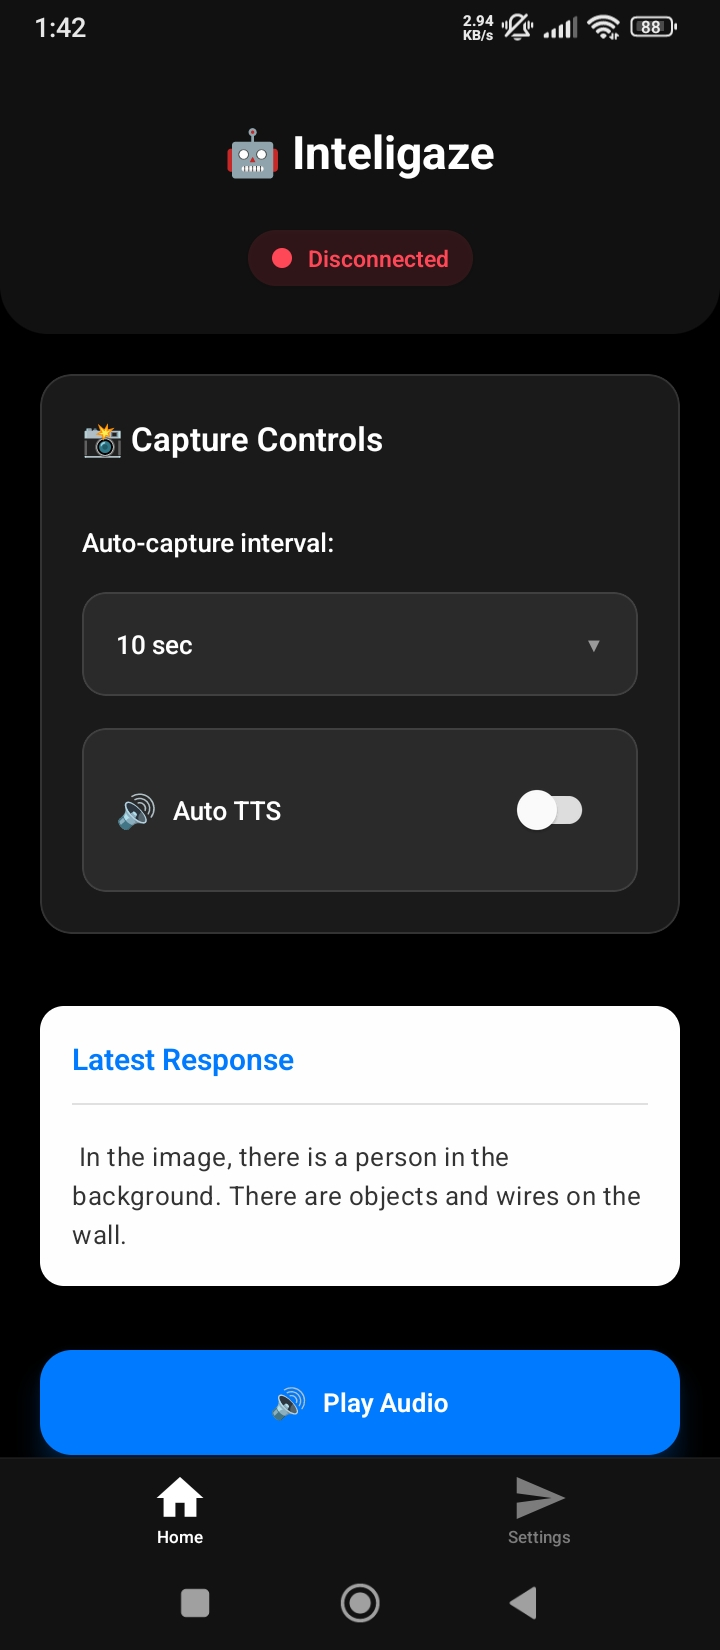
\includegraphics[width=0.4\textwidth]{fig/mobile_vision_main.jpg}
    \caption{Mobile App: Main Vision Screen}
    \label{fig:mobile_vision_screen}
\end{figure}
\textbf{Key elements visible/functional on this screen include:}
\begin{itemize}
    \item \textbf{Title:} "AI Vision Assistant".
    \item \textbf{Vision Status Bar (\texttt{VisionStatusBar}):} Displays "Connected" or "Disconnected" based on ESP32 camera feed status from the backend.
    \item \textbf{Backend Status:} Indicates if the app can reach the FastAPI backend (implicitly shown if controls are active and status bar updates).
    \item \textbf{Capture Controls (\texttt{CaptureControls}):}
        \begin{itemize}
            \item "Capture Now" button (if not in auto-capture mode).
            \item "Auto-capture" switch.
            \item If auto-capture is enabled: Interval selection (e.g., "5 sec") and "Auto TTS" switch.
        \end{itemize}
    \item \textbf{Loading Indicator:} Appears when an image is being processed by the AI.
    \item \textbf{Response Card (\texttt{ResponseCard}):} Displays the latest textual description from the AI.
    \item \textbf{Play TTS Button:} Appears below the response if not in full auto-TTS mode, allowing manual playback of the latest response.
    \item \textbf{History List (\texttt{HistoryList}):} Shows a scrollable list of previous AI descriptions with timestamps.
    \item \textbf{Log Panel (\texttt{LogPanel}):} An expandable panel showing system event logs.
\end{itemize}

\subsection{Settings Screen (\texttt{settings.tsx})}
Figure \ref{fig:mobile_settings_screen} shows the settings configuration screen.
\begin{figure}[H]
    \centering
    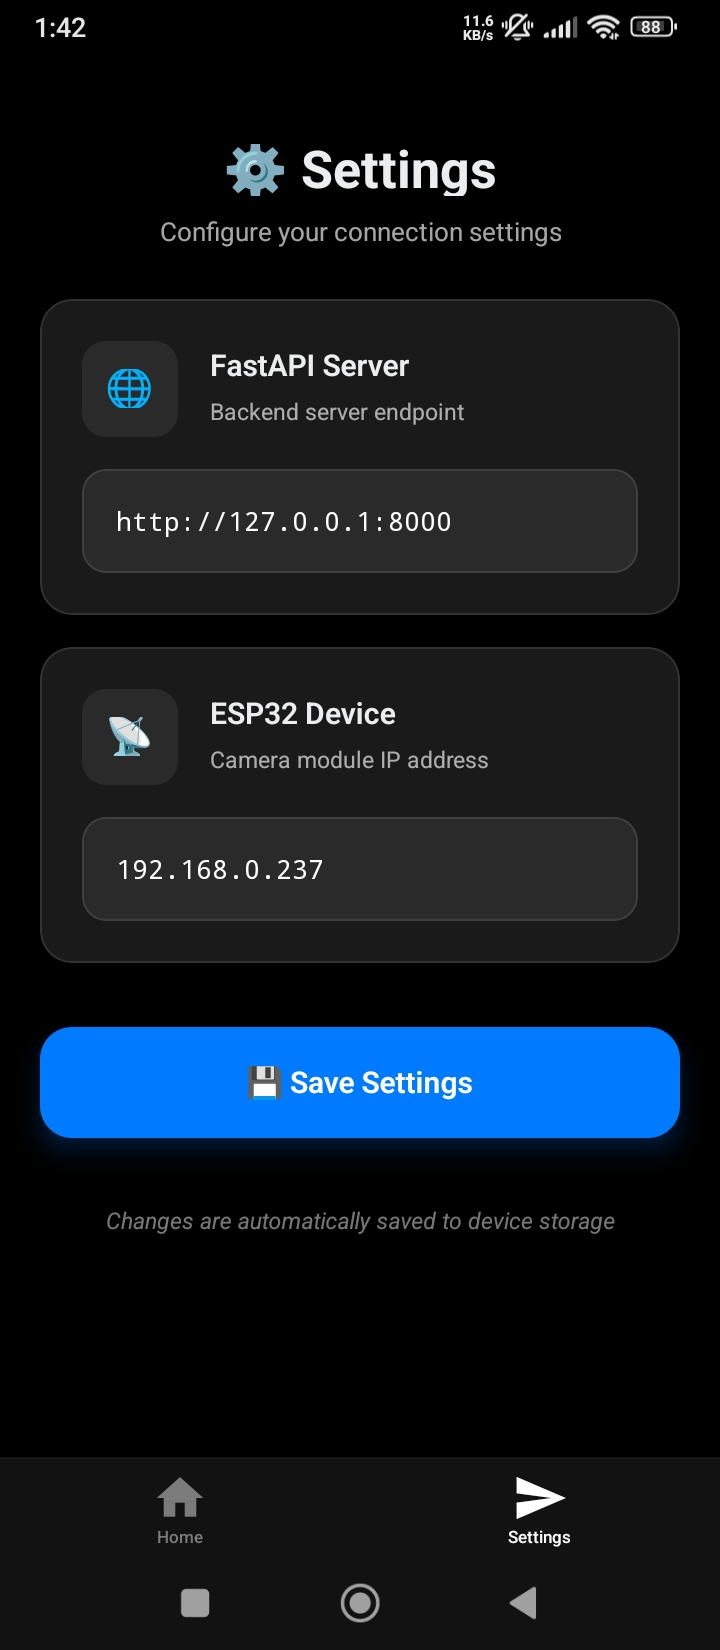
\includegraphics[width=0.4\textwidth]{fig/mobile_settings.jpg}
    \caption{Mobile App: Settings Screen}
    \label{fig:mobile_settings_screen}
\end{figure}
Users can:
\begin{itemize}
    \item Set the "FastAPI Server URL" (e.g., `http://192.168.0.213:8000`).
    \item Set the "ESP32 IP Address" (e.g., `192.168.0.237`). This IP is for reference or for direct connection if the app logic were to change, as the FastAPI server currently has its own ESP32 IP.
    \item Save these settings, which are stored locally using AsyncStorage.
\end{itemize}

\section{Desktop Application Showcase (\texttt{Desktop/app.py})}
The PyQt6 desktop application provides an alternative interface.
Figure \ref{fig:desktop-main-screen} illustrates the main window of the desktop application.
\begin{figure}[H]
    \centering
    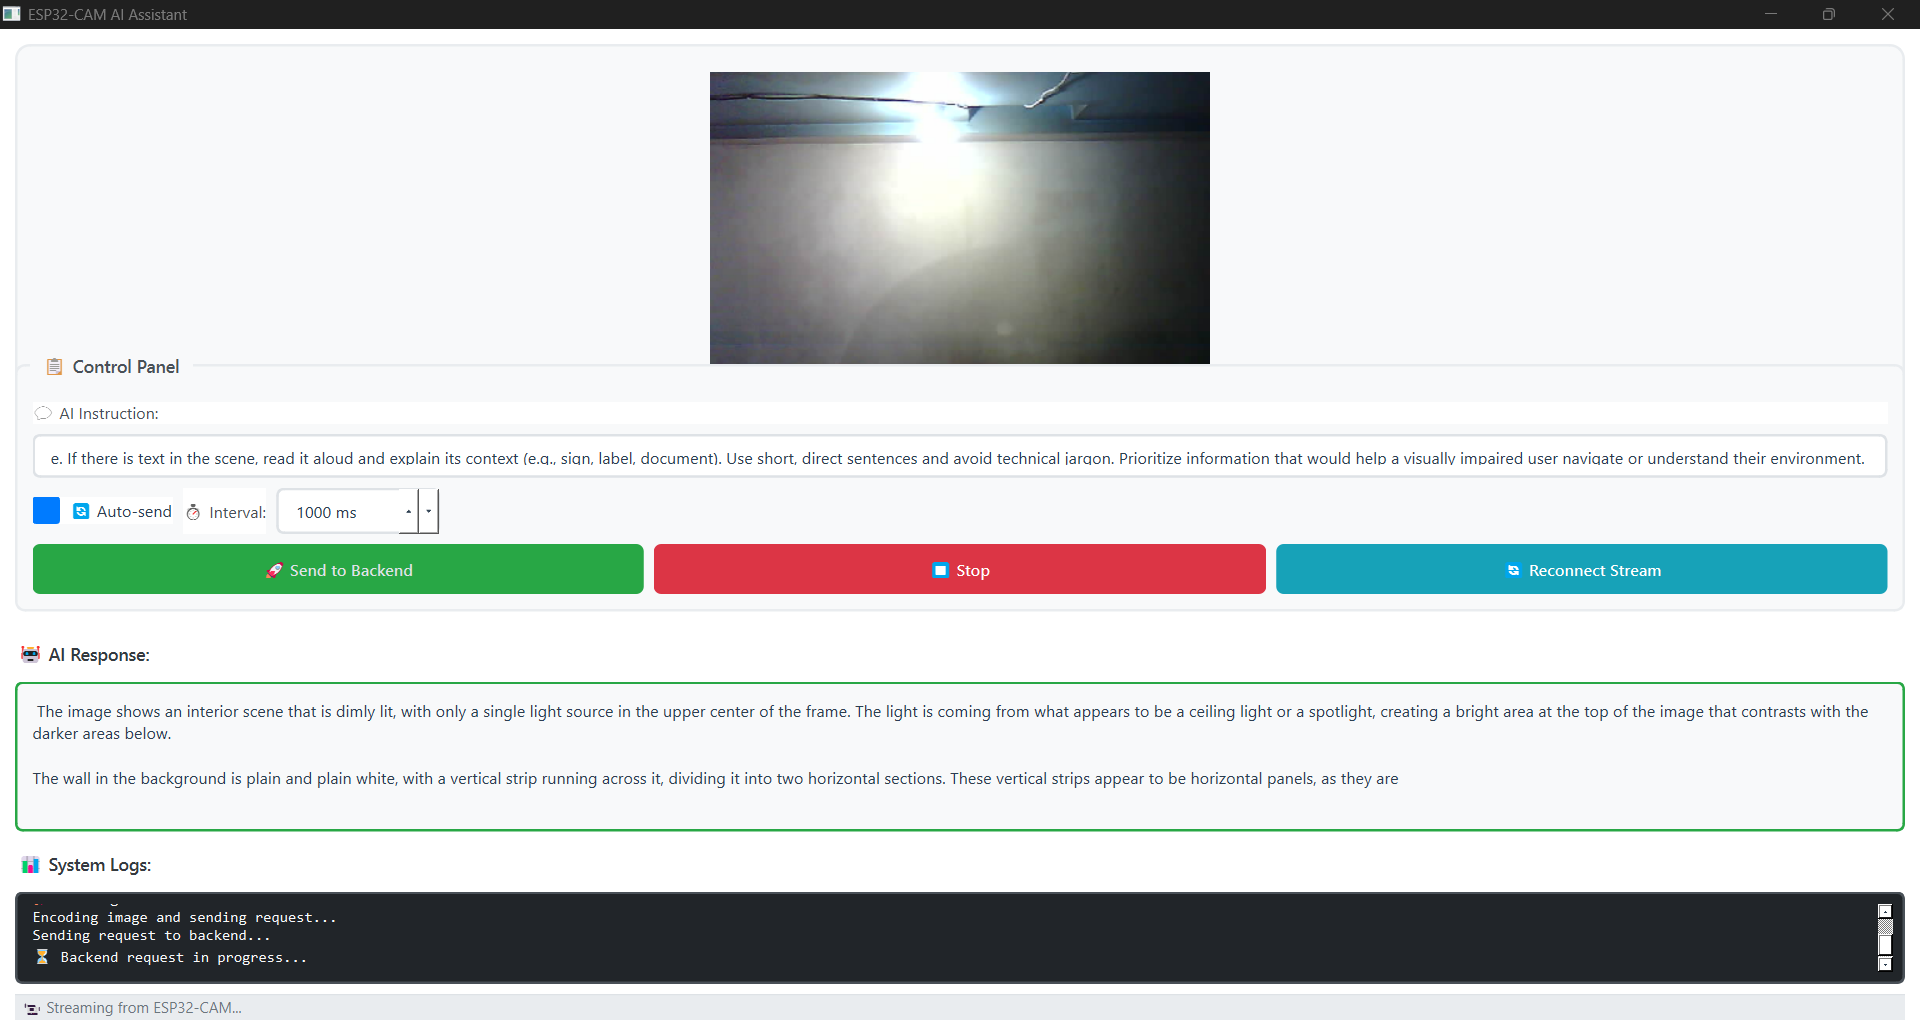
\includegraphics[width=0.9\textwidth]{fig/desktop-main.png}
    \caption{Desktop App: Main Window}
    \label{fig:desktop-main-screen}
\end{figure}
\textbf{Key elements visible/functional on this screen include:}
\begin{itemize}
    \item \textbf{Video Feed Area:} Displays the live video from the ESP32-CAM (or local webcam if configured).
    \item \textbf{Instruction Input Field:} Pre-filled with `DEFAULT\_INSTRUCTION`, editable by the user.
    \item \textbf{Controls Group:}
        \begin{itemize}
            \item "Auto-send" checkbox and interval spinbox (e.g., "1000 ms").
            \item "Send to Backend" button.
            \item "Stop" button (to halt auto-send or ongoing requests).
            \item "Reconnect Stream" button (to re-initialize the ESP32 stream connection).
        \end{itemize}
    \item \textbf{Backend Response Area:} A text edit box displaying the latest AI-generated description.
    \item \textbf{Logs Area:} A text edit box displaying system logs and status messages.
    \item \textbf{Status Bar:} Shows current operational status (e.g., "Streaming from ESP32-CAM...", "Backend response received.").
\end{itemize}

\section{Key Feature Walkthrough}
\subsection{Manual Capture and AI Description}
\begin{enumerate}
    \item \textbf{Mobile:} User taps "Capture Now". App sends request to FastAPI server. Server gets latest ESP32 frame from its internal cache, sends to AI. AI response displayed on mobile.
    \item \textbf{Desktop:} User clicks "Send to Backend". App gets current ESP32 frame directly from its stream, sends directly to the AI vision service. AI response displayed on desktop.
\end{enumerate}
\textit{Expected Result:} A concise textual description of the scene currently viewed by the camera appears in the respective response area. For example, if the camera sees a desk with a laptop, the response might be: "The image shows a desk with a silver laptop on it. There is also a black mouse to the right of the laptop."

\subsection{Auto-Capture with Auto-TTS (Mobile App)}
\begin{enumerate}
    \item User enables "Auto-capture" and "Auto TTS" switches, and selects an interval (though the interval is mainly for the non-TTS auto-capture; TTS-chained mode proceeds after TTS finishes).
    \item App starts capturing frames by sending requests to the FastAPI server.
    \item After each capture, the AI description is received from the server.
    \item The description is automatically played via Text-to-Speech using the Groq TTS service.
    \item Once TTS playback completes (or after a short buffer), the next capture cycle begins by sending another request.
\end{enumerate}
\textit{Expected Result:} The user continuously hears descriptions of their changing surroundings as they move the wearable camera, facilitating hands-free operation.

\subsection{Performance Observations (User to fill with actual data)}
\begin{itemize}
    \item \textbf{ESP32 Stream Latency:} (e.g., Visually observed on desktop app, generally low on local network, typically <1 second for frame to appear).
    \item \textbf{AI Response Time (Mobile App via Server):} Average time from "Capture Now" tap to response display. (e.g., Typically 500-1650 ms depending on network and AI service load).
    \item \textbf{AI Response Time (Desktop App Direct):} Average time from "Send to Backend" click to response display. (e.g., Typically 300-1270 ms, potentially slightly faster due to one less hop).
    \item \textbf{TTS Generation and Playback Latency (Mobile App):} Time from receiving AI text to start of audio playback. (e.g., Typically 1-3 seconds for Groq API call and audio processing).
\end{itemize}

% --- CHAPTER 6: CONCLUSION AND FUTURE WORK ---
\chapter{Conclusion and Future Work}
\section{Conclusion}
The IntelliGaze project successfully developed and demonstrated a functional prototype of a wearable AI camera system designed to assist visually impaired individuals. The system effectively integrates an ESP32-CAM for real-time video input, a FastAPI backend for processing and AI interfacing (primarily for the mobile client), and user-friendly client applications (React Native mobile and PyQt6 desktop) for interaction and feedback. The desktop client also demonstrates direct AI service interaction.

The project achieved its primary objectives:
\begin{itemize}
    \item A live video stream was successfully established from the ESP32-CAM.
    \item AI-powered scene interpretation was implemented, providing textual descriptions of visual input by leveraging a cloud-based vision service and carefully engineered prompts.
    \item Intuitive user feedback mechanisms were created, including textual display and Text-to-Speech output on the mobile platform.
    \item Versatile client applications were developed, catering to both mobile and desktop use cases, with features like manual/auto capture, response history, and system logging.
    \item The system architecture exhibits modularity, and key parameters are configurable, demonstrating a flexible design.
\end{itemize}
IntelliGaze showcases the potential of combining modern embedded systems, web technologies, and AI to create meaningful assistive solutions. The use of optimized prompts tailored for accessibility proved crucial in generating relevant and helpful descriptions. While a prototype, it lays a solid foundation for a more robust and feature-rich assistive device. The architectural choice of having the desktop client interact directly with the AI service, while the mobile client uses an intermediary FastAPI server, offers different trade-offs and was an interesting aspect of the development.

\section{Future Work}
Building upon the current IntelliGaze prototype, several avenues for future development and enhancement are identified:
\begin{itemize}
    \item \textbf{Enhanced AI Models and On-Device Processing:}
        \begin{itemize}
            \item Explore newer, more powerful, or specialized multimodal AI models for improved accuracy, faster response times, and more nuanced descriptions (e.g., recognizing specific product brands, understanding more complex scenes).
            \item Investigate the feasibility of running smaller, optimized AI models directly on more powerful edge devices (e.g., Raspberry Pi, Jetson Nano, or next-gen ESP32 variants with AI capabilities) to reduce reliance on cloud services, decrease latency, and improve privacy.
        \end{itemize}
    \item \textbf{Improved Hardware Integration:}
        \begin{itemize}
            \item Integrate higher-resolution camera sensors with better low-light performance.
            \item Incorporate depth sensors (e.g., LiDAR, ToF sensors) to provide 3D environmental understanding for better obstacle avoidance and navigation cues.
            \item Add haptic feedback mechanisms (e.g., vibration motors) to convey alerts or directional information discreetly.
            \item Focus on power optimization and compact, ergonomic wearable design, including battery integration.
        \end{itemize}
    \item \textbf{Advanced Feature Development:}
        \begin{itemize}
            \item \textbf{Interactive Q\&A:} Allow users to ask follow-up questions about the scene (e.g., "What color is the car?", "How many people are there?"). This would require maintaining context with the AI service.
            \item \textbf{Navigation Assistance:} Integrate with GPS and mapping services to provide basic orientation and turn-by-turn directions contextualized with visual information.
            \item \textbf{Personalized Object/Face Recognition:} Allow users to train the system to recognize specific personal items or familiar faces (with strong emphasis on privacy and consent mechanisms).
            \item \textbf{Offline Mode:} Develop limited offline capabilities, perhaps using smaller on-device models for basic object recognition if cloud connectivity is lost.
        \end{itemize}
    \item \textbf{Robustness, Security, and Usability:}
        \begin{itemize}
            \item Implement comprehensive error handling and recovery mechanisms across all system components.
            \item Enhance security: Move API keys (like Groq's) from client-side code to the backend server. Implement authentication for API endpoints if exposing the server more broadly. Use HTTPS for all communications.
            \item Conduct thorough usability testing with visually impaired users to gather feedback and iteratively improve the UI/UX of both mobile and desktop applications, focusing on accessibility standards.
            \item Improve battery management for the wearable unit and provide clear battery status indicators.
        \end{itemize}
    \item \textbf{Streamline Backend Interaction:} Consider unifying client interaction through the FastAPI server to centralize AI logic, API key management, and potentially caching, especially if the web client is further developed. This would require the server to handle image uploads or direct image data from clients other than its ESP32 stream.
    \item \textbf{Full Web Client Development:} Expand the existing `web/` prototype into a fully functional web-based client, offering another access point to the system, possibly also leveraging the FastAPI backend.
    \item \textbf{Community and Open Source:} Consider releasing parts of the project as open-source to foster community contributions and wider adoption.
\end{itemize}
These future directions aim to evolve IntelliGaze into a more powerful, reliable, and indispensable tool for enhancing the independence and quality of life for visually impaired individuals.

% --- CHAPTER 7: PROJECT MANAGEMENT ---
\chapter{Project Management}

\section{Team Contributions}

The IntelliGaze project was brought to fruition through dedicated effort, with team members focusing on various components under a cohesive development strategy. The specific contributions are detailed below:

\begin{itemize}
    \item \textbf{Touhidul Alam Seyam (230240003):}
    \begin{itemize}
        \item Served as the project lead and chief architect, spearheading the overall design, development, and end-to-end integration of the IntelliGaze system.
        \item Led the development of the React Native mobile application, including its UI/UX, core logic, state management, navigation (Expo Router), and communication with backend services.
        \item Drove the integration of all system components: the ESP32 camera feed, FastAPI backend server, mobile and desktop client applications, and external AI vision and TTS services.
        \item Played a crucial role in troubleshooting and resolving complex technical challenges across the entire system.
        \item Managed the project's version control (Git), repository organization, and contributed significantly to the initial drafts and final compilation of project documentation and this lab report.
        \item Oversaw hardware selection, initial setup, and the integration aspects of hardware with software components.
    \end{itemize}

    \item \textbf{Shafiul Azam Mahin (230240022):}
    \begin{itemize}
        \item Focused on the development of the PyQt6 desktop application (\texttt{Desktop/app.py}).
        \item This involved designing the graphical user interface, implementing the display of the video feed from the ESP32 or webcam, and developing the logic for direct communication with the AI vision service using the \texttt{BackendThread}.
        \item Handled event loops, threading for non-blocking operations, and signal/slot mechanisms specific to the desktop application's UI updates.
    \end{itemize}

    \item \textbf{Eftakar Uddin (230240004):}
    \begin{itemize}
        \item Contributed to the development of the FastAPI backend server framework (\texttt{Flask\_server/server.py}).
        \item Responsibilities included implementing the API endpoints (\texttt{/status}, \texttt{/vision}), structuring the server logic to handle client requests, and managing server-side error handling and logging mechanisms.
    \end{itemize}

    \item \textbf{Muntasir Rahman (230240002):}
    \begin{itemize}
        \item Concentrated on the ESP32-CAM firmware development (\texttt{camera-feed.ino}).
        \item This involved programming the microcontroller for camera initialization, establishing WiFi connectivity, and implementing the MJPEG streaming logic to provide the live video feed.
    \end{itemize}

    \item \textbf{Tasmim Akther Mim (230240025):}
    \begin{itemize}
        \item Focused on integrating the Text-to-Speech (TTS) functionality within the mobile application.
        \item This involved implementing the \texttt{playGroqTTS.ts} utility to interface with the Groq TTS API, enabling the system to provide auditory feedback of the AI-generated descriptions.
    \end{itemize}
\end{itemize}

All team members actively participated in brainstorming sessions, problem-solving, debugging, and the overall testing phases of the project. Regular meetings were held to discuss progress and address challenges.

\section{Gantt Chart}
The project was managed according to a predefined schedule, outlining key phases, tasks, and deadlines. Figure \ref{fig:gantt_chart} presents the Gantt chart illustrating the project timeline.
\begin{figure}[H]
    \centering
    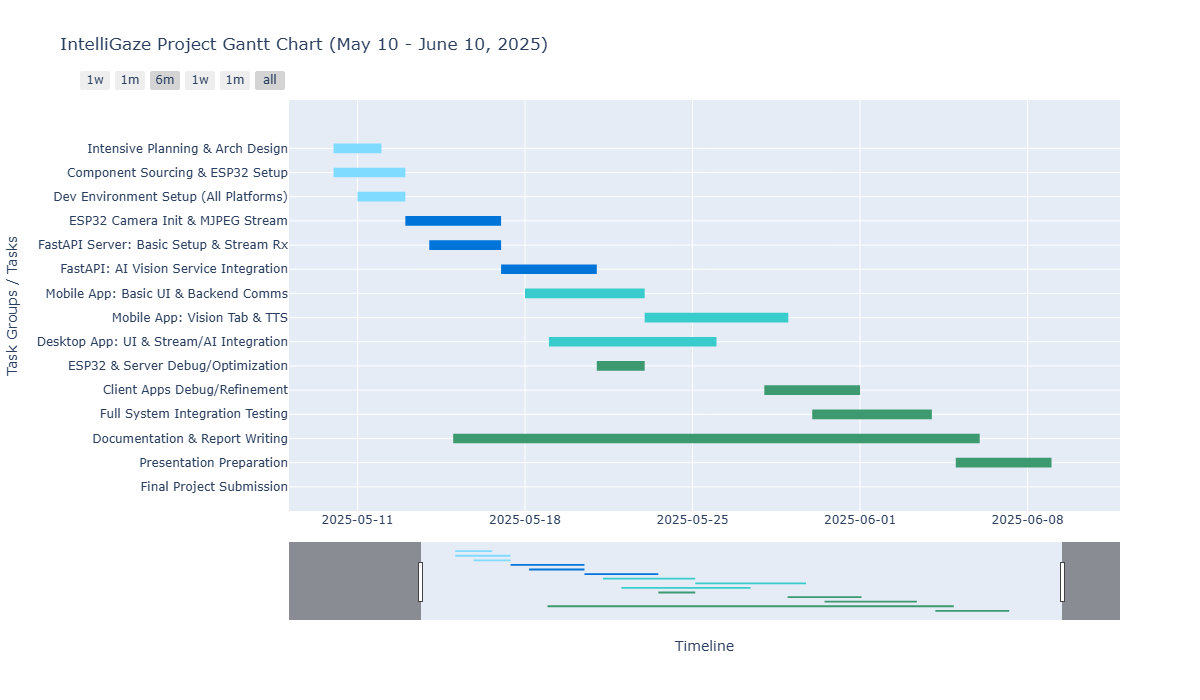
\includegraphics[height=0.85\textwidth, angle=90]{fig/gantt_chart.png}
    \caption{Project Gantt Chart}
    \label{fig:gantt_chart}
\end{figure}


\textit{The project timeline, as depicted in Figure \ref{fig:gantt_chart}, spanned approximately one month. The initial phase, from around May 11th to May 16th, focused on \textbf{Intensive Planning \& Architecture Design}, \textbf{Component Sourcing \& ESP32 Setup}, and establishing the \textbf{Development Environment} for all platforms.
Following this, from roughly May 15th to May 22nd, the core hardware and backend development took place, including \textbf{ESP32 Camera Initialization \& MJPEG Streaming}, \textbf{FastAPI Server Basic Setup \& Stream Reception}, and \textbf{FastAPI AI Vision Service Integration}.
Client application development occurred largely in parallel from approximately May 20th to May 29th, encompassing \textbf{Mobile App Basic UI \& Backend Communications}, the \textbf{Mobile App Vision Tab \& TTS} features, and the \textbf{Desktop App UI \& Stream/AI Integration}.
A dedicated period for \textbf{ESP32 \& Server Debugging/Optimization} was scheduled around May 24th-26th, followed by \textbf{Client Apps Debugging/Refinement} from May 27th to June 1st, and \textbf{Full System Integration Testing} from May 29th to June 3rd.
\textbf{Documentation \& Report Writing} was an ongoing task from mid-May (around May 18th) through June 6th. The final stages involved \textbf{Presentation Preparation} (June 4th-8th) leading up to the \textbf{Final Project Submission} around June 10th, 2025.}


% --- REFERENCES ---
\cleardoublepage
\begin{thebibliography}{99}
    \bibitem{fastapi}
    Tiangolo. (n.d.). \textit{FastAPI}. FastAPI Documentation. Retrieved May 20, 2025, from \url{https://fastapi.tiangolo.com/}

    \bibitem{reactnative}
    Meta Platforms, Inc. (n.d.). \textit{React Native – A framework for building native apps with React}. React Native Documentation. Retrieved May 20, 2025, from \url{https://reactnative.dev/}

    \bibitem{pyqt6}
    Riverbank Computing. (n.d.). \textit{Introduction to PyQt6}. PyQt6 Documentation. Retrieved May 20, 2025, from \url{https://www.riverbankcomputing.com/static/Docs/PyQt6/}

    \bibitem{esp32arduino}
    Espressif Systems. (n.d.). \textit{Arduino ESP32 Core}. GitHub Repository. Retrieved May 20, 2025, from \url{https://github.com/espressif/arduino-esp32}

    \bibitem{opencv}
    OpenCV team. (n.d.). \textit{OpenCV (Open Source Computer Vision Library)}. OpenCV Official Site. Retrieved May 20, 2025, from \url{https://opencv.org/}
    
    \bibitem{axios}
    Axios Community. (n.d.). \textit{Axios - Promise based HTTP client for the browser and node.js}. GitHub Repository. Retrieved May 20, 2025, from \url{https://github.com/axios/axios}

    \bibitem{expo}
    Expo. (n.d.). \textit{Expo - Make apps with React}. Expo Documentation. Retrieved May 20, 2025, from \url{https://docs.expo.dev/}

    \bibitem{groqapi}
    Groq. (n.d.). \textit{Groq API Documentation}. GroqCloud Console. Retrieved May 20, 2025, from \url{https://console.groq.com/docs}

    \bibitem{esp32cam_datasheet}
    AI-Thinker. (n.d.). \textit{ESP32-CAM Development Board Datasheet}. (Typically found via distributors or AI-Thinker's website, provide specific URL if available).

    \bibitem{python}
    Python Software Foundation. (n.d.). \textit{Python Language Reference}. Python.org. Retrieved May 20, 2025, from \url{https://www.python.org}
    
    
    \bibitem{gemma3blog1_google}
    Google. (2024, May). \textit{Gemma 3 outperforms other models in its class}. Google Blog. Retrieved May 20, 2025, from \url{https://blog.google/technology/developers/gemma-3/}

    \bibitem{gemma3blog2_devs}
    Google Developers. (2024, May). \textit{Introducing Gemma 3}. Google Developers Blog. Retrieved May 20, 2025, from \url{https://developers.googleblog.com/en/introducing-gemma3/}
\end{thebibliography}

% --- APPENDIX ---
\cleardoublepage % Ensures appendix starts on a new page, and is odd if two-sided
\appendix
\chapter{Project Directory Structure}
\label{app:directory_structure}

The IntelliGaze project is organized into several main directories, each containing specific components of the system. The high-level structure is as follows:

\begin{verbatim}
camera-feed/            # ESP32-CAM Firmware
  camera-feed.ino/
    camera-feed.ino
Desktop/                # PyQt6 Desktop Application
  app.py/
    app.py
Flask_server/           # FastAPI Backend Server
  server.py/
    server.py
inteligaze/             # React Native Mobile Application (Expo)
  .gitignore
  .vscode/
    settings.json/
  app/                  # Expo Router app directory
    _layout.tsx
    (tabs)/             # Tab-based navigation setup
      _layout.tsx
      explore.tsx
      index.tsx
      settings.tsx
      vision.tsx
    +not-found.tsx
  app.json              # Expo configuration file
  assets/               # Static assets (fonts, images) - (Inferred, not explicitly in list but typical)
  components/           # Reusable React Native components
    CaptureControls.tsx
    Collapsible.tsx
    ... (other UI components) ...
    ui/                 # More specific UI elements (Card, IconSymbol)
  constants/            # Global constants (e.g., Colors.ts)
  hooks/                # Custom React hooks
  scripts/              # Utility scripts (e.g., reset-project.js)
  utils/                # Utility functions (e.g., playGroqTTS.ts)
  package.json          # NPM package dependencies and scripts
  README.md
  tsconfig.json         # TypeScript configuration
Test/                   # Test scripts and files
  index.html            # HTML test page for vision endpoint
  test_fastapi.py       # Python script to test FastAPI server
  test.py               # Python script for image upload test
web/                    # Web Client Prototype
  index.html
  script.js
  style.css
\end{verbatim}

\chapter{Key Configuration Files}
\label{app:config_files}

\section{Expo Configuration (\texttt{inteligaze/app.json})}
This file configures the Expo build and runtime environment for the React Native mobile application.
\begin{lstlisting}[language=Python, caption={Snippet from inteligaze/app.json}, basicstyle=\ttfamily\tiny\linespread{0.9}]
{
  "expo": {
    "name": "inteligaze",
    "slug": "inteligaze",
    "version": "1.0.0",
    "orientation": "portrait",
    "icon": "./assets/images/icon.png",
    "scheme": "inteligaze",
    "userInterfaceStyle": "automatic",
    "newArchEnabled": true,
    "ios": {
      "supportsTablet": true
    },
    "android": {
      "adaptiveIcon": {
        "foregroundImage": "./assets/images/adaptive-icon.png",
        "backgroundColor": "#ffffff"
      },
      "edgeToEdgeEnabled": true
    },
    "web": {
      "bundler": "metro",
      "output": "static",
      "favicon": "./assets/images/favicon.png"
    },
    "plugins": [
      "expo-router",
      [
        "expo-splash-screen",
        {
          "image": "./assets/images/splash-icon.png",
          "imageWidth": 200,
          "resizeMode": "contain",
          "backgroundColor": "#ffffff"
        }
      ],
      "expo-audio"
    ],
    "experiments": {
      "typedRoutes": true
    }
  }
}
\end{lstlisting}

\section{React Native Dependencies (\texttt{inteligaze/package.json})}
The main dependencies for the mobile application are listed here.
\begin{lstlisting}[language=Python, caption={Dependencies from inteligaze/package.json}, basicstyle=\ttfamily\tiny\linespread{0.9}]
{
  "dependencies": {
    "@expo/vector-icons": "^14.1.0",
    "@react-native-async-storage/async-storage": "2.1.2",
    "@react-navigation/bottom-tabs": "^7.3.10",
    "@react-navigation/elements": "^2.3.8",
    "@react-navigation/native": "^7.1.6",
    "axios": "^1.9.0",
    "expo": "~53.0.9",
    "expo-audio": "~0.4.5",
    "expo-av": "~15.1.4",
    "expo-blur": "~14.1.4",
    "expo-constants": "~17.1.6",
    "expo-font": "~13.3.1",
    "expo-haptics": "~14.1.4",
    "expo-image": "~2.1.7",
    "expo-linking": "~7.1.5",
    "expo-router": "~5.0.6",
    "expo-splash-screen": "~0.30.8",
    "expo-status-bar": "~2.2.3",
    "expo-symbols": "~0.4.4",
    "expo-system-ui": "~5.0.7",
    "expo-web-browser": "~14.1.6",
    "react": "19.0.0",
    "react-dom": "19.0.0",
    "react-native": "0.79.2",
    "react-native-gesture-handler": "~2.24.0",
    "react-native-reanimated": "~3.17.4",
    "react-native-safe-area-context": "5.4.0",
    "react-native-screens": "~4.10.0",
    "react-native-web": "~0.20.0",
    "react-native-webview": "13.13.5"
  }
}
\end{lstlisting}


\chapter{Core Software Libraries and Frameworks}
\label{app:libraries}
This section lists the primary software libraries and frameworks utilized in the development of each major component of the IntelliGaze system.

\section{ESP32-CAM Firmware (\texttt{camera-feed.ino})}
\begin{itemize}
    \item \textbf{Arduino Core for ESP32:} Base platform for ESP32 development.
    \item \textbf{\texttt{WiFi.h}:} For WiFi connectivity.
    \item \textbf{\texttt{esp\_camera.h}:} For interfacing with the ESP32 camera module.
    \item \textbf{\texttt{esp\_http\_server.h}:} For creating the HTTP server to stream MJPEG.
    \item \textbf{\texttt{esp\_timer.h}:} For timer functionalities (though not explicitly used for complex timing in the provided snippet, it's a core ESP-IDF component).
\end{itemize}

\section{FastAPI Backend Server (\texttt{Flask\_server/server.py})}
\begin{itemize}
    \item \textbf{Python 3:} Core programming language.
    \item \textbf{FastAPI:} Modern, fast (high-performance) web framework for building APIs.
    \item \textbf{Uvicorn:} ASGI server to run FastAPI applications.
    \item \textbf{HTTPX:} Asynchronous HTTP client for making requests to the ESP32 stream and the external AI vision service.
    \item \textbf{Loguru:} Library for pleasant and powerful logging.
    \item \textbf{OpenCV-Python (\texttt{cv2}):} Used for decoding and potentially processing image frames from the ESP32 (though direct processing is minimal in the current server logic, it's used for validation).
    \item \textbf{Pydantic:} For data validation and settings management (used implicitly by FastAPI for request/response models).
    \item \textbf{Base64, Time, Threading:} Standard Python libraries.
\end{itemize}

\section{React Native Mobile Application (\texttt{inteligaze/})}
\begin{itemize}
    \item \textbf{React Native:} Framework for building native mobile applications using JavaScript/TypeScript and React.
    \item \textbf{Expo:} Platform and toolset for building universal React applications (iOS, Android, Web).
        \begin{itemize}
            \item \textbf{Expo Router:} File-system based routing.
            \item \textbf{Expo Audio/AV (\texttt{expo-av}):} For playing audio (TTS).
            \item \textbf{Expo FileSystem (\texttt{expo-file-system}):} For saving temporary audio files.
            \item \textbf{Expo Haptics, Expo Image, Expo Linking, Expo SplashScreen, Expo StatusBar, Expo Symbols, Expo WebBrowser, Expo Constants, Expo Font, Expo Blur, Expo SystemUI}
        \end{itemize}
    \item \textbf{TypeScript:} Superset of JavaScript adding static typing.
    \item \textbf{Axios:} Promise-based HTTP client for making API requests to the backend and Groq TTS.
    \item \textbf{React Navigation (\texttt{@react-navigation/*}):} For navigation between screens and tabs.
    \item \textbf{AsyncStorage (\texttt{@react-native-async-storage/async-storage}):} For persistent local storage (settings).
    \item \textbf{React Native Reanimated, React Native Gesture Handler, React Native Safe Area Context, React Native Screens, React Native WebView}
\end{itemize}

\section{PyQt6 Desktop Application (\texttt{Desktop/app.py})}
\begin{itemize}
    \item \textbf{Python 3:} Core programming language.
    \item \textbf{PyQt6:} Set of Python bindings for Qt 6, used for creating the graphical user interface.
    \item \textbf{OpenCV-Python (\texttt{cv2}):} For fetching and processing (encoding/decoding) video frames from the ESP32 or webcam.
    \item \textbf{Requests:} Synchronous HTTP client for making requests to the external AI vision service.
    \item \textbf{NumPy:} For numerical operations, often used with OpenCV.
    \item \textbf{Base64, Sys, Threading (QThread):} Standard Python libraries and PyQt threading.
\end{itemize}


\end{document}